\newif\ifdraft %XXX
\drafttrue % \draftfalse %XXX

%%%--- Template for master thesis at SfS
%%%--- Modified template with more comments and examples -- SG, 11/06/09
%%%------
\ifdraft \documentclass[11pt,a4paper]{report} \else%XXX
\documentclass[11pt,a4paper,twoside,openright]{report}
\fi %XXX
\usepackage[english]{sty/ETHDAsfs}%--> ETHDASA + fancyhdr + ... "umlaute"
%  + sfs-hyper -> hyperref 

\usepackage{pdfpages}%%to include the confirmation of originality (plagiarism
\usepackage{amsbsy}%% for \boldsymbol and \pmb{.}
\usepackage{amssymb}%% calls  amsfonts...
\usepackage{graphicx}%-- für PostScript-Grafiken (besser als  psfig!)
%\usepackage[draft]{graphicx} % grafics shown as boxes --> faster compilation
%
\usepackage[longnamesfirst]{natbib}%was {sfsbib}%- Für  Literatur-Referenzen
%           ^^^^^^^^^^^^^^ 1) "Hampel, Ronchetti, ..,"  2) "Hampel et al"
% Engineers (and other funny people) want to see [1], [2] 
% ---> use 'numbers' : \usepackage[longnamesfirst,number]{natbib}
%
%
\usepackage{sty/texab}%- 'tex Abkürzungen' /u/sfs/tex/tex/latex/texab.sty
        %%- z.B.  \R, \Z, \Q, \Nat für reelle, ganze, rationale, natürl. Zahlen;
        %%-       \N   (Normalvert.)  \W == Wahrscheinlichkeit .....
        %%-  \med, \var, \Cov, \....
        %%-  \abs{x} == |x|   und   \norm{y} ==  || y ||   (aber anständig)
%% NOTE: texab contains many useful definitions and "shortcuts". It is
%% worth to open the file and have a look at them. HOWEVER, some
%% definitions are a bit can lead to conflicts with other packages. You
%% might for example want to comment out the line defininf \IF as an
%% operator when working with the algorithmic package, or to comment out
%% the line defining a command \Cite with working with the Biblatex package  
\usepackage{amsmath}
%\usepackage{mathrsfs}% Raph Smith's Formal Script font --> provides \mathscr
\usepackage[utf8]{inputenc}% <<------- Unicode, *NOT* iso-latin1 !
\usepackage{ae}% A[lmost] E[uropean] Fonts
\usepackage{enumerate}% Fuer selbstdefinierte Nummerierungen
%--------
\usepackage{relsize}%-> \smaller (etc) used here
\usepackage{color} %% to allow coloring in code listings
\usepackage{pgf}
\usepackage{listings}% Fuer R-code, C-code, ....  and settings for these:
% listings
  \definecolor{Mygrey}{gray}{0.75}% for linenumbers and only!
  \definecolor{Cgrey}{gray}{0.4}% for comments
  \lstloadlanguages{R}
  %%--- first version of "listings of R"-style : ---------------------------
  % %% using \smaller here: makes R code listings use a *small* font:
  % \lstset{language=R,basicstyle=\smaller[2],commentstyle=\rmfamily\smaller,
  %   showstringspaces=false,xleftmargin=4ex,
  %   literate={<-}{{$\leftarrow$}}1 {~}{{$\sim$}}1}
  % \lstset{escapeinside={(*}{*)}} % for (*\ref{ }*) inside lstlistings (Scode) 
  %\newcommand{\lil}[1]{\lstinline|#1|}
  %%--- newer version of "listings of R"-style : ---------------------------
  \lstset{%% Help, e.g. --> https://en.wikibooks.org/wiki/LaTeX/Source_Code_Listings
    language=R,
    basicstyle=\ttfamily\scriptsize,%%- \small > \footnotesize > \scriptsize > \tiny
    %commentstyle=\ttfamily\color{Cgrey},
    commentstyle=\itshape\color{Cgrey},
    numbers=left,
    numberstyle=\ttfamily\color{Mygrey}\tiny,
    stepnumber=1,
    numbersep=5pt,
    backgroundcolor=\color{white},
    showspaces=false,
    showstringspaces=false,
    showtabs=false,
    frame=single,
    tabsize=2,
    captionpos=b,
    breaklines=true,
    %breakatwhitespace=false,
    keywordstyle={},
    morekeywords={},
    xleftmargin=4ex, 
    literate={<-}{{$\leftarrow$}}1 {~}{{$\sim$}}1
  }
  \lstset{escapeinside={(*}{*)}} % for (*\ref{ }*) inside lstlistings (Scode) 
%%----------------------------------------------------------------------------

%%------- Theoreme ---
\newtheorem{definition}{Definition}[subsection]
\newtheorem{lemma}[definition]{Lemma}
\newtheorem{theorem}[definition]{Theorem}
\newtheorem{Coro}[definition]{Corollary}
\theoremstyle{definition} 
\newtheorem{example}[definition]{Example}
\newtheorem*{note}{Note}
\newtheorem*{remark}{Remark}

\DeclareMathOperator*{\plim}{plim}
% \def\MR#1{\href{http://www.ams.org/mathscinet-getitem?mr=#1}{MR#1}}

% \newcommand{\Lecture}[3]{\marginpar{#3.#2.#1}}
% \newcommand{\Fu}{\mathcal{F}}
\newcommand{\aatop}[2]{\genfrac{}{}{0pt}{}{#1}{#2}}

%\renewcommand{\theequation}{\arabic{equation}}
\numberwithin{equation}{subsection}

%%%%%%%%%%%%%%%%%%%%%%%%%%%%%%%%%%%%%%%%%%%%%%%%%
%%% Path for your figures                      %%%
%%%%%%%%%%%%%%%%%%%%%%%%%%%%%%%%%%%%%%%%%%%%%%%%%
% Set the paths where all figures are taken from:
\graphicspath{{./figures/}}

%%%%%%%%%%%%%%%%%%%%%%%%%%%%%%%%%%%%%%%%%%%%%%%%%
%%% Define your own commands here             %%%
%%%%%%%%%%%%%%%%%%%%%%%%%%%%%%%%%%%%%%%%%%%%%%%%%
\newcommand{\Bruch}[2]{{}^{#1}\!\!/\!_{#2}}
\renewcommand{\labelenumi}{\roman{enumi}.)}
\ifdraft \usepackage{lineno} \linenumbers  %XXX
\definecolor{mygray}{gray}{0.75}
\renewcommand{\linenumberfont}{\normalfont\scriptsize\color{mygray}}
\fi %XXX

\usepackage{my_modifications}


\begin{document}
\bibliographystyle{chicago}% ---> Hampel,F., E.Ronchetti,... W.Stahel(1986) ...
%was \bibliographystyle{sfsbib}\citationstyle{dcu} %OR DEFAULT : \citationstyle{agsm}

\pagenumbering{roman}%- roman numbering for first few pages

%%%%%%%%%%%%%%%%%%%%%%%%%%%%%%%%%%%%%%%%%%%%%%%%%
%%% Title page                                %%%
%%%%%%%%%%%%%%%%%%%%%%%%%%%%%%%%%%%%%%%%%%%%%%%%%
\period{Spring 2022}
\dasatype{Master Thesis}
\students{Lukas Graz}
\mainreaderprefix{Adviser:}
\mainreader{Prof.\ Dr.\ Nicolai Meinshausen}
\alternatereaderprefix{Co-Adviser:}
\alternatereader{Gregor Perich}
\submissiondate{September 18th 2022}
\title{Interpolation and Correction \\ of \\ Multispectral Satellite Image Time Series}

\maketitle%- Titelseite wird abgeschlossen
\ifdraft \else%XXX
  \cleardoublepage
\fi %XXX
%%~~~~~~~~~~~~~~~~~~~~~~~~~~~~~~~~~~~~~~~~

%%%%%%%%%%%%%%%%%%%%%%%%%%%%%%%%%%%%%%%%%%%%%%%%%
%%% Insert here acknowledgements and abstract %%%
%%%%%%%%%%%%%%%%%%%%%%%%%%%%%%%%%%%%%%%%%%%%%%%%%
%% Dedication (optional)

  % \markright{}
  % \vspace*{\stretch{1}}
  % \begin{center}
  %   To some special person
  % \end{center}
  % \vspace*{\stretch{2}}

  % Preface (optional)
  \newpage
  \markboth{Preface}{Preface}
  \chapter*{Preface}

First words and acknowledgements.

XXX

Betreuung von Gregor

Ideen mit Meinshausen

Resourccen vom SFS

%%% Local Variables: 
%%% mode: latex
%%% TeX-master: "MasterThesisSfS"
%%% End: 


  % Abstract should not be longer than one page.
  \newpage
  \markboth{Abstract}{Abstract}
  \chapter*{Abstract}

%% Intro
Multispectral satellite imagery is used to model vegetation characteristics and development on a large scale in agriculture. As an example, satellite-derived Time Series (TS) of spectral indices like the Normalized Difference Vegetation Index (NDVI) are used to classify crops and to predict crop yield. 
%% Problem Illustration
Sometimes satellite measurements do not match the ground signal due to contamination by clouds and other atmospheric effects. Therefore, traditional approaches aim to filter out contaminated observations before extracting and subsequently interpolating the NDVI. After filtering, remaining contaminated observations and resulting data gaps are the two challenges for interpolation that we address in this thesis.
%% Our Setting
For this purpose, cereal crop yield maps from 2017-2021 of a farm in Switzerland with the corresponding Sentinel 2 satellite image TS published by the European Space Agency were examined. Contaminated observations were filtered with the provided Scene Classification Layer (SCL). 
%% NDVI itpl
We give a benchmark-supported review of different interpolation methods. Based on it, we found Smoothing Splines as a flexible non-parametric method and Double Logistic approximation as a parametric method with implicit shape assumptions to perform most favorably given the aforementioned challenges. In addition, we generalize an iterative technique which robustifies interpolation methods against outliers by reducing their weights. In most cases, this robustification successfully decreased the 50\% and 75\% quantiles of the absolute out-of-bag residuals. 
%% NDVI corr. 
Moreover, we present a general interpolation procedure that utilizes additional information to correct the target variable with an uncertainty estimate and then performs a weighted interpolation. In our setting, the target variable is the NDVI and as additional information we use the SCL, the observed NDVI and the spectral bands. Consequently, we no longer filter using the SCL, but weight observations according to their reliability. % The combination of different interpolation methods and correction models yields 28 interpolation strategies. % To choose the best one, we assume that, the better the interpolated NDVI TS models crop growth, the more suitable it is to predict crop yield. 
% {The resulting interpolation strategy uses Smoothing Splines and corrects the NDVI with uncertainty estimation through a simple linear model considering only of the observed NDVI and the associated SCL class.} 
Applying this procedure, the unexplained variance in crop yield estimations via the resulting NDVI TS decreased by~10.5\%. 
% Impact
Considering the success of the presented procedure with respect to NDVI TS, it appears promising for applications to other satellite-based TS given its cloud-correcting properties.

% %% Reproducibility  +  R-package
% Instructions and a codebase for reproducibility of the results, as well as an R package making the presented general interpolation procedure accessible to the user, are supplied. 



%%% Local Variables: 
%%% mode: latex
%%% TeX-master: "MasterThesisSfS"
%%% End: 


%%%%%%%%%%%%%%%%%%%%%%%%%%%%%%%%%%%%%%%%%%%%%%%%%
%%% Table of contents and list of figures and %%%   
%%% tables (no need to change this usually)   %%%
%%%%%%%%%%%%%%%%%%%%%%%%%%%%%%%%%%%%%%%%%%%%%%%%%
\newpage
\tableofcontents
\listoftodos
\ifdraft 
\else%XXX
  % \newpage
  % \listoffigures
  % \newpage
  % \listoftables

  %% Notations and glossary (optional)
  \cleardoublepage
\fi
\phantomsection
\addcontentsline{toc}{chapter}{\protect\numberline{}{Notation}}
\markboth{Notation}{Notation}
\chapter*{\vspace{-3.2cm} Notations}
\label{c:Notation}
\vspace{-0.6cm}
Since this thesis, despite its applied nauture, is located at the Mathematics Department, we adhere to the convention of speaking in the first person plural ``we''.\\
Moreover, only equations that are referenced elsewhere are equipped with a number.

\section*{Variables}\vspace{-0.2cm}
\renewcommand{\arraystretch}{1.3} % for non-dense tables
\begin{longtable}{p{0.12\linewidth} p{0.87\linewidth}}
$c$		& a (vector of) constant(s)\\
$\lambda \in \R$		& a scalar\\
$n\in \mathbb{N}$		& sample size\\
$i,j$		& indices in $\{1,\dots,n\}$\\
$n\in \R^n$		& time, usually in GDD\\
$w \in \R^n$		& a vector of weights for each location $x$\\
$y\in \R^n$		& response in 1-dim interpolation setting\\
$\hat y\in \R^n$		& estimate of $y$\\
$\bar y\in \R$		& sample mean of $y$\\
$r \in \R^n$		& residuals given by $y - \hat y$\\
$X\in\R^{n\times p}$ & the design matrix. Each row corresponds to one observation and each column to one covariate.\\
$X_{[:,j]}$ 	& the $j$-th column of $X$\\
$X_{[i,:]}$ 	& the $i$-th row of $X$
% $x\in \R^n$		& covariable in 1-dim interpolation setting
\end{longtable}

%%%%%%%%%%%%%%%%%%%%%%%%%%%
\section*{Abbreviations and Objects}\vspace{-0.2cm}
\begin{longtable}{p{0.12\linewidth} p{0.87\linewidth}}
NDVI	
		& Normalized Difference Vegetation Index \citep{rouseMonitoringVernalAdvancement1974}.\\

TS	
		& Time Series. \\
IM	
		& Interpolation Method. That is a simple\footnote{I.e., no combination of various methods.} method that interpolates data $(t_i,y_i)_{i = 1,\dots ,n}$ and yields a function $f(t)=y$, approximating the data. \\
IS	
		& Interpolation Strategy. This is the category of functions that map $(t_i,y_i)_{i=1,\dots,n}$ to a function $f(t)=y$, approximating the data. So a IS describes a strategy of how to arrive at an interpolation starting from the data $(t_i,y_i)_{i=1,\dots,n}$. For this, initial data may be corrected (cf. chapter~\ref{sec:corr}), (possible different) IMs (iteratively) used, weightings applied (cf. robustification in section~\ref{sec:loess_robustify}). Note, that strictly speaking every IM also is an IS. But usually we expect an IS to involve a more `complex' procedure. \\
S2	
		& Sentinel 2 satellites. Two multi-spectral image satellites deployed by the European Space Agency. \\
SCL	
		& Scene Classification Layer provided by the European Space Agency that gives an estimation of the land cover class of each pixel. It indicates what one can expect at a pixel at a sampled time. For an overview, see table~\ref{tab:satelite/scl_classes}\\
Pixel	
		& A pixel originates of an image pixel and describes a square of 10 x 10 meters in the field that coincides with the resolution (and location) of the Sentinel-2 pixels. Such pixels are illustrated in figure~\ref{fig:satelite/witzwil_2021_P112_yield_cropped.png}. Additional information like yield is also attached.\\

$P_t$	
		& the observed data (weather and spectral bands) at time $t$ and the location of one pixel. \\

$P$	
		& a pixel. We see it as a collection of all the observations at the specified location within one season. More formally, $P := \left\{P_t | t\text{ is a valid sample time within a defined season}\right\}$\\


$P^{SCL45}$	
		& is similar to $P$ but we only consider observations that belong to the classes 4 and 5. This is used done to get a subset of observations which are less contaminated by clouds and shadows.\\

DAS	
		& Days After Sowing\\

GDD	
		& Growing Degree Days -- cumulative sum of ``$\max(0, \text{temperature}-\text{threshold})$''\\

YPE 	
		& (Relative) Yiepld Prediction Error. See Definition~\ref{def:YPE}\\

OOB 	
		& Out Of the Box. Describes the procedure of  estimating the value for a point by a model that has not seen this point before (see section~\ref{sec:OOB_LOOCV}).\\

LOOCV 	
		& Leave One Out Cross Validation. Describes the procedure of estimating the value for a point by a model that has seen all the points except the current one (see section~\ref{sec:OOB_LOOCV}).
\end{longtable} 

\section*{Statistical Models}\vspace{-0.2cm}
\begin{longtable}{p{0.12\linewidth} p{0.87\linewidth}}
	DL
		& Double Logistic (see section~\ref{sec:double_logistic})\\
	FS
		& Fourier Series (see section~\ref{sec:fourier_approx})\\
	NW
		& Nadaraya-Watson (see section~\ref{sec:Kernel})\\
	UK
		& Universal Kriging (see section~\ref{sec:Kriging})\\
	SG
		& Savitzky-Golay Filter (see section~\ref{sec:Savitzky-Golay})\\
	LOESS
		& Locally Weighted Regression (see section~\ref{sec:loess})\\
	BS
		& B-splines (see section~\ref{sec:B})\\
	SS
		& Smoothing Splines (see section~\ref{sec:Natural_SS})\\
	OLS
		& Ordinary Least Squares (see section~\ref{sec:corr_model_OLS})\\
	OLS\textsuperscript{SCL}
		& OLS using only the observed NDVI and SCL classes (as factor variables)\\
	OLS\textsuperscript{all}
		& OLS using the covarietes OLS\textsuperscript{SCL} uses and the spectral bands\\
	LASSO
		& Least Absolute Shrinkage and Selection Operator (see section~\ref{sec:corr_model_LASSO})\\
	GAM
		& General Additive Model (see section~\ref{sec:corr_model_GAM})\\
	RF
		& Random Forest (see section~\ref{sec:corr_model_RF})\\
	MARS
		& Multivariate Adaptive Regression Splines (see section~\ref{sec:corr_model_MARS})\\
\end{longtable} \renewcommand{\arraystretch}{1}

% \bigskip











%%% Local Variables: 
%%% mode: latex
%%% TeX-master: "MasterThesisSfS"
%%% End: 


\ifdraft \else%XXX
  \cleardoublepage
\fi %XXX
\pagenumbering{arabic}%--- switch back to standard numbering 


%%%%%%%%%%%%%%%%%%%%%%%%%%%%%%%%%%%%%%%%%%%%%%%%%
%%% Your text... Either write here directly,  %%%
%%% or even better: write in separate files   %%%
%%% that you just have to include here.       %%% 
%%%%%%%%%%%%%%%%%%%%%%%%%%%%%%%%%%%%%%%%%%%%%%%%%
\chapter{Introduction}

Remote sensing aims to measure target variables efficiently from a distance. 
% stakeholders + applications  
Large scale monitoring of forest and agricultural vegetation dynamics is of great interest to authorities, insurance companies and research. Examples include crop classification for subsidizing farmers \citep{henitsSentinel2EnablesNationwide2022} and the creation of crop models for estimating crop yields or nitrogen concentrations \citep{couraultSTICSCropModel2021,perichCropNitrogenRetrieval2021}. 
% Season Start (start of spring) (community name: land surface plant phenology)
For this, freely distributed multi-spectral satellite imagery from the  Sentinel-2 (S2) satellites are examined \citep{esaSentinel22022}.
% NDVI
In order to transform the high dimensional satellite images into easily interpretable metrics, spectral indices such as the Normalized Difference Vegetation Index (NDVI) are used \citep{rouseMonitoringVernalAdvancement1974}. The NDVI serves as a proxy for photosynthetic activity \citep{gamonRelationshipsNDVICanopy1995a}, and thus the corresponding {NDVI Time Series ({TS})} reflects the vegetation development. 
% S2 issues (clouds ...)
The quality of a satellite image, however, depends on atmospheric conditions. Thus, in case of a dense cloud cover, the information content derived from the NDVI is impaired. Therefore, \cite{esaEuropeanSpaceAgency2022} also provides a Scene Classification Layer (SCL), which provides additional metadata about what is observed (e.g., shadows, clouds, vegetation, etc.) . So when extracting the NDVI {TS} from the Sentinel 2 satellite imagery {TS}, we can filter out the contaminated observations using the SCL classification. However, due to this filtration it may occur that we have no observations for several weeks, especially in winter. It is also possible that some observations are wrongly classified by the SCL (e.g., as vegetation) and thus result in an outlier in the NDVI TS. Consequently, the main challenge is to interpolate an NDVI {TS}, which can contain large data gaps and outliers. 

% state-of-the-art
Currently, there are several approaches to address these issues. One is to look at the observed evolution of the canopy coverage and assume its bell shape for the NDVI {TS} given the strong correlation between NDVI and photosynthetic activity. Approaches to model this include a \nth{2} order Fourier approximation \citep{stockliEuropeanPlantPhenology2004} or a Double Logistic function \citep{beckImprovedMonitoringVegetation2006}.
On the other hand, assumptions are made about more abstract properties of the curve, such as smoothness. We divide these into local and global approaches. Nadaraya-Watson \citep{strbacEstimationEvapotrasnpirationUrban2017}, Savitzky-Golay Filter \citep{chenSimpleMethodReconstructing2004a} and Locally Reweighed Regression \citep{omoriAssessmentPaddyFields2021} use a sliding window to interpolate the {TS} stepwise. Global methods like B-Splines \citep{gurungPredictingEnhancedVegetation2009} and Smoothing Splines \citep{caiPerformanceSmoothingMethods2017} reduce the squares of all residuals simultaneously, and Universal Kriging fits a Gaussian process to the data \citep{chandolaScalableTimeSeries2010}.
% SS defined in \cite{cravenSmoothingNoisyData1978}

\pagebreak
The research questions pursued in this thesis are:
\begin{Nenumerate}
    \item Which {{IM}}s are used in the context of NDVI, and what are their advantages and disadvantages?
    \item How may contaminated data be dealt with?
    \item How do data gaps affect interpolation?
    \item How to deal with data gaps?
    \item How can we recognize a good interpolation of the NDVI?
\end{Nenumerate}
\bigskip



% our contribution + roadmap:
In this thesis, we will discuss the strengths and weaknesses of Interpolation Methods ({{IM}}s) and evaluate them with respect to NDVI interpolation. For this purpose, we use the Sentinel 2 satellite image {TS} and crop yield maps of different fields of different cereal species on a farm in Witzwil, Switzerland over the years 2017-2021. After presenting the available data, illustrating challenges and defining different concepts in chapter~\ref{sec:data_methods} (\nameref{sec:data_methods}), we turn to the two main blocks of this thesis. One covers the study of IMs and the other presents a general procedure of correcting (NDVI) TS with uncertainty estimation by utilizing additional information.
On the first block, in chapter~\ref{sec:itpl} (\nameref{sec:itpl}) we examine parametric and non-parametric {{IM}}s and discuss their strengths and weaknesses (question i.). We generalize and test an iterative technique that makes IMs more robust to outliers by weighting them less (question ii.). To evaluate IMs, we present an approach that uses out-of-bag residuals (question v.). In section~\ref{sec:discussion_itpl_data_gaps} (\nameref{sec:discussion_itpl_data_gaps}), we discuss how different {{IM}}s respond to data gaps (question iii.), and in section~\ref{sec:itpl_preselection} (\nameref{sec:itpl_preselection}) we preselect {{IM}}s. This preselection, we evaluate in the results section~\ref{sec:results_itpl} (\nameref{sec:results_itpl}) and select two candidates from the {{IM}}s in section~\ref{sec:itpl_candiate_selection} (\nameref{sec:itpl_candiate_selection}).
For the second block, we correct possibly contaminated data with statistical models in chapter~\ref{sec:corr} (\nameref{sec:corr}) (question ii.) and utilize previously ignored observations, which we hope will further reduce data gaps (question iv.). Thus, we no longer filter the observations a priori via the SCL, but instead correct the observed NDVI and weight the observations via estimated uncertainties. By combining different statistical models and IMs, we obtain 28 Interpolation Strategies ({{ISs}}). We compare those with a vegetation-oriented quality measure (question v.) and describe the results in section~\ref{sec:results_ndvi_corr} (\nameref{sec:results_ndvi_corr}). Based on these results, in section~\ref{sec:discussion_corr} (\nameref{sec:discussion_corr}) we argue what the best {{IS}} is. In addition, we justify why our NDVI correction can be understood as unsupervised learning and why we relied only on satellite imagery and not on meteorological data for the NDVI correction.
Our conclusions of this thesis, recommendations, as well as an outlook on future work is given in chapter~\ref{sec:Conclusion} (\nameref{sec:Conclusion}). 


% und Definieren verschiedene Konzepte. Darunter eine transformation der Zeitachse, welche datenlücken im Winter zusammenschrumpfen lässt (Frage iv.). 




%smoothing:   ``Similarly, smoothing the {TS} of satellite data is helpful to address inconsistency in observation frequency and timing due to clouds and other sensor artefacts \cite{skakunWinterWheatYield2019}''


%%% Local Variables: 
%%% mode: latex
%%% TeX-master: "MasterThesisSfS"
%%% End: 

\chapter{Problem Description}

\section{Available Data}
	{
		Our study region is a farm of over 800ha, which is located in western Switzerland. From REF-gregor we acquire satellite image data (section \ref{sec:s2_img_data}), yield maps of several cereals from 2017 to 2021 (section \ref{sec:yieldmapping_data}), and meteorological data (section \ref{sec:gather_data_to_pixel}).
	}

	\subsection{Sentinel 2 Satellite Image Data}{
		\label{sec:s2_img_data}
		\subsubsection*{General Information}{
			The European Space Agency (ESA) \footnote{REF: https://sentinel.esa.int/web/sentinel/missions/sentinel-2} freely distributes the high quality images of the two Sentinel satellites 2 (S2). Together, both satellites have a revisit time of 5 days at the equator and 2-3 at mid-latitudes. However, at our study region we only receive an image every 5 days.
			In order to decrease the effect of atmospheric conditions like reflections and scattering, we will not work with the raw data but with the results of the Level-2A processing\footnote{REF https://sentinels.copernicus.eu/web/sentinel/technical-guides/sentinel-2-msi/level-2a/algorithm}\footnote{XXXREF gregor perich ``Data prior to March 2018 was only145
			available in the top-of-atmosphere L1C format and was downloaded as such [...] L1C data was processed to L2A product level using the `Sen2Cor' processor provided by ESA''}. 
		}

		\subsubsection*{Data Description}{
			The Level-2A processed images we use contain 12 spectral bands with local resolutions up to 10 meters (see \ref{table:S2-bands}).   
			\begin{table}[h]
    \centering
    \small
    \caption{List of spectral bands of the S2-satellites. Each band has its center at the wavelength $\lambda$ in $nm$ with the spectral width $\Delta\lambda$ in $nm$ with a spatial resolution $SR$ in $m$ \citep{jaramazESASentinel2Mission2013}.}
    \begin{tabular}{p{0.03\linewidth} p{0.04\linewidth} p{0.03\linewidth} p{0.03\linewidth} p{0.73\linewidth}}
    \toprule
        \hspace*{-5pt} Band & $\;\lambda$ & $\Delta\lambda$ & $SR$ & Purpose \\ \hline
        1 & 443 & 20 & 60 & Atmospheric correction (aerosol scattering) \\ %\hline
        2 & 490 & 65 & 10 & Sensitive to vegetation senescing, carotenoid, browning and soil background; atmospheric correction (aerosol scattering) \\ %\hline
        3 & 560 & 35 & 10 & Green peak, sensitive to total chlorophyll in vegetation \\ %\hline
        4 & 665 & 30 & 10 & Maximum chlorophyll absorption \\ %\hline
        5 & 705 & 15 & 20 & Position of red edge; consolidation of atmospheric corrections / fluorescence baseline. \\ %\hline
        6 & 740 & 15 & 20 & Position of red edge, atmospheric correction, retrieval of aerosol load. \\ %\hline
        7 & 783 & 20 & 20 & Leaf Area Index (LAI), edge of the Near-Infrared (NIR) plateau. \\ %\hline
        8 & 842 & 115 & 10 & LAI \\ %\hline
        8a & 865 & 20 & 20 & NIR plateau, sensitive to total chlorophyll, biomass, LAI and protein; water vapor absorption reference; retrieval of aerosol load and type. \\ %\hline
        9 & 945 & 20 & 60 & Water vapor absorption, atmospheric correction. \\ %\hline
        10 & 1375 & 30 & 60 & Detection of thin cirrus for atmospheric correction. \\ %\hline
        11 & 1610 & 90 & 20 & Sensitive to lignin, starch and forest above ground biomass. Snow/ice/cloud separation. \\ %\hline
        12 & 2190 & 180 & 20 & Assessment of Mediterranean vegetation conditions. Distinction of clay soils for the monitoring of soil erosion. Distinction between live biomass, dead biomass and soil, e.g., for burn scars mapping. \\
        \bottomrule
    \end{tabular}
    \label{table:S2-bands}
\end{table}

			Bands which have a lower resolution (20 and 60 meters) will be scaled up to 10 meters using cubic interpolation (REF gregor perich).
							% \begin{figure}[h]
							% 	\label{fig:satelite/sentinel-2-bands}
							% 	\center
							% 	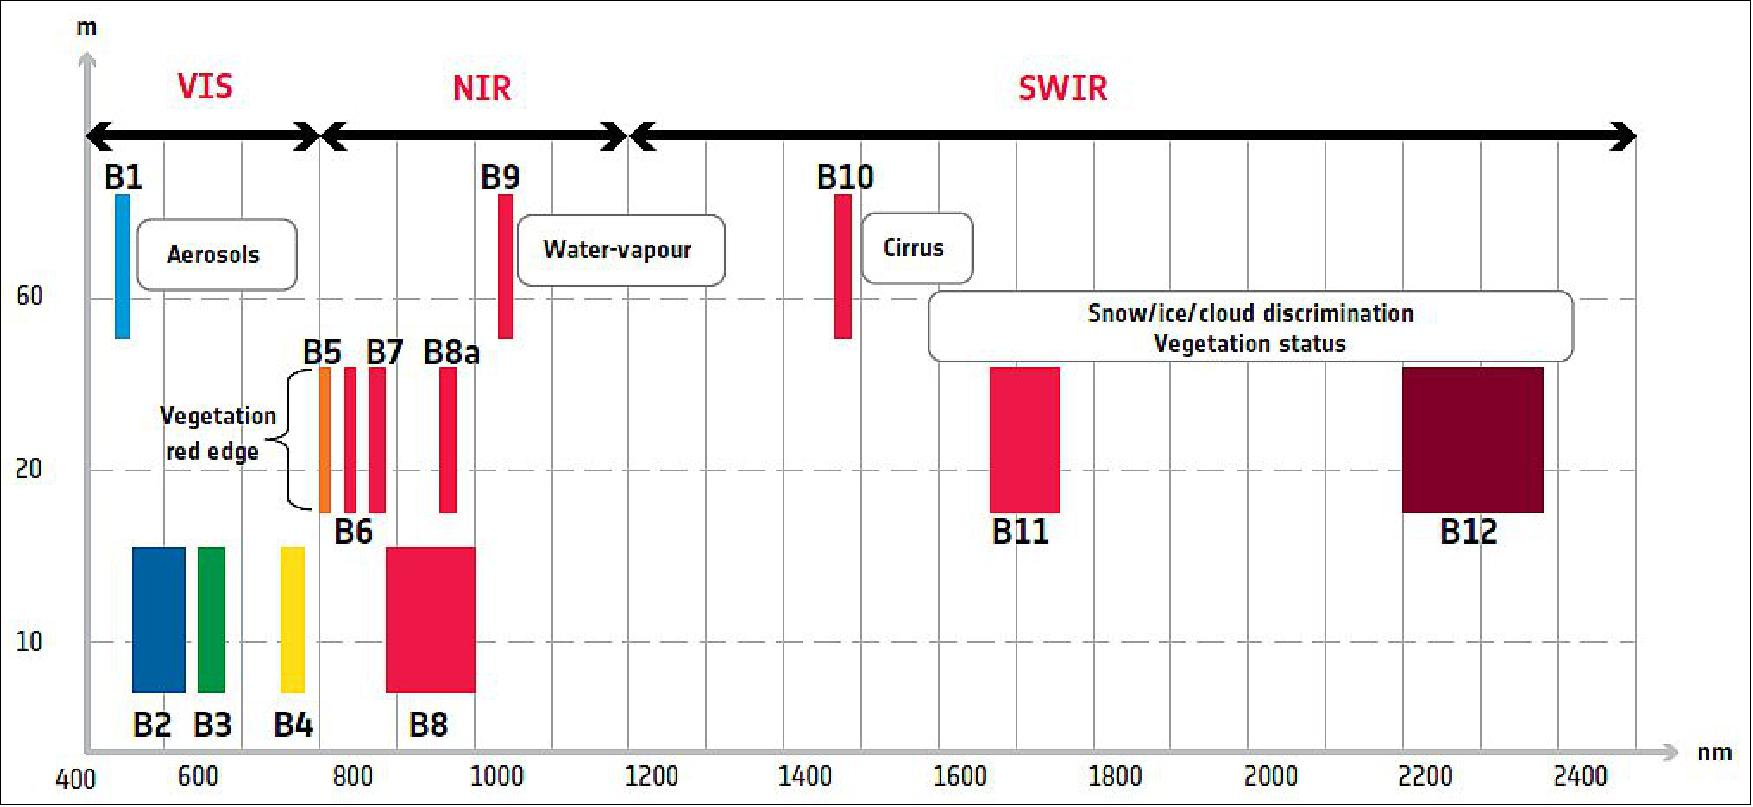
\includegraphics[width=0.4\textwidth]{satelite/sentinel-2-bands.jpg}
							% 	\caption{XXX Sentinel 2 bands}
							% \end{figure}
			Additional to the spectral bands the ESA also supplies a Scene Classification Layer (\textit{SCL}) where for each location the observed subject is assigned to an \textit{SCL-class} (cf. table~\ref{tab:satelite/scl_classes}). In chapter \ref{sec:itpl}  we will use this classification to filter out unreliable data points considering only SCL-classes 4 and 5.  
			
			
			\begin{table}[h]
				\caption{Overview: Scene Classification Layers (SCL)}
				\label{tab:satelite/scl_classes}
				\center
				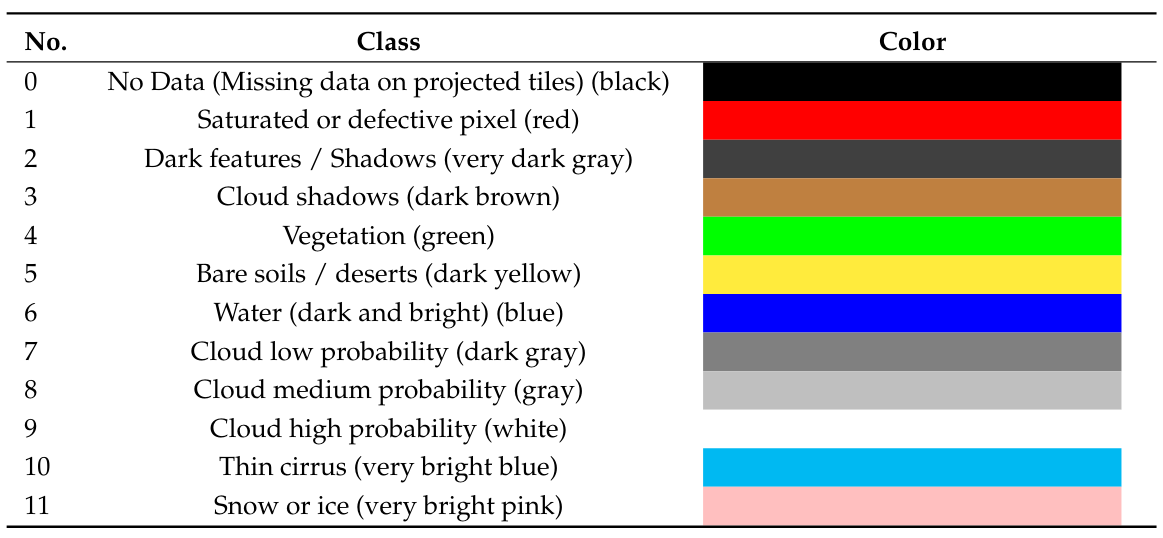
\includegraphics[width=0.8\textwidth]{satelite/scl_classes.png}
			\end{table}
		}

		\subsubsection*{Data Illustration}{
				%satelite/time_series_2021_P112/15_scl5_2021-02-23.png
	%satelite/time_series_2021_P112/30_scl4_2021-05-09.png
	%satelite/time_series_2021_P112/33_scl9_2021-05-24.png
	%satelite/time_series_2021_P112/35_scl4_2021-06-03.png
	%satelite/time_series_2021_P112/40_scl10_2021-06-28.png
	%satelite/time_series_2021_P112/45_scl2_2021-07-23.png

\begin{figure*}
	\centering
	\begin{subfigure}[b]{0.31\textwidth}
		\centering
		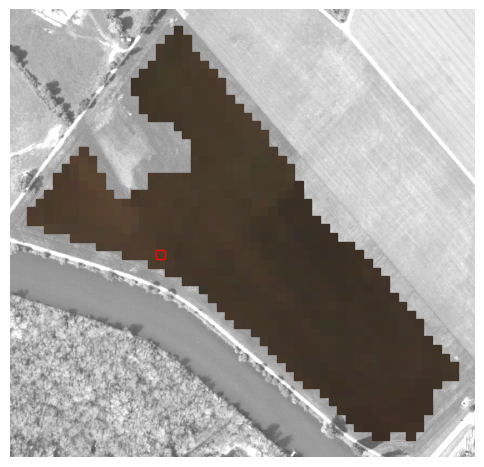
\includegraphics[width=\textwidth]{satelite/time_series_2021_P112/15_scl5_2021-02-23.png}
		\caption[2021-02-23\hspace*{0.1cm} SCL 5]%
		{{\small 2021-02-23\hspace*{0.1cm} SCL 5}}    
		\label{fig:satelite/time_series_2021_P112/15_scl5_2021-02-23.png}
	\end{subfigure}
	\hfill
	\begin{subfigure}[b]{0.31\textwidth}  
		\centering 
		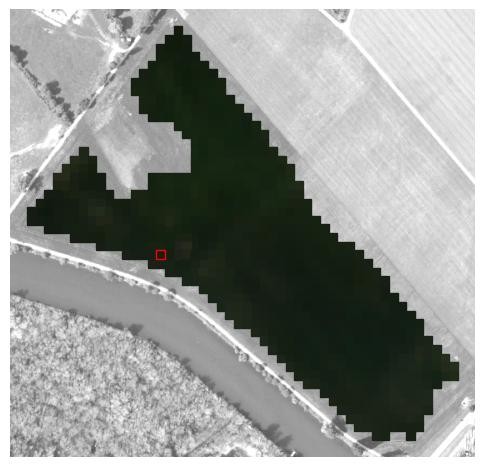
\includegraphics[width=\textwidth]{satelite/time_series_2021_P112/30_scl4_2021-05-09.png}
		\caption[2021-05-09\hspace*{0.1cm} SCL 4]%
		{{\small 2021-05-09\hspace*{0.1cm} SCL 4}}    
		\label{fig:satelite/time_series_2021_P112/30_scl4_2021-05-09.png}
	\end{subfigure}
	\hfill
	\begin{subfigure}[b]{0.31\textwidth}  
		\centering 
		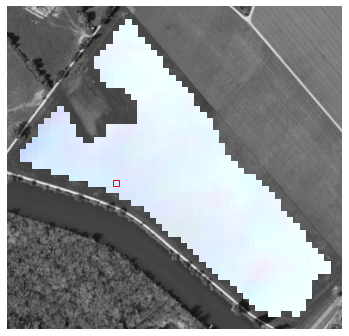
\includegraphics[width=\textwidth]{satelite/time_series_2021_P112/33_scl9_2021-05-24.png}
		\caption[2021-05-24\hspace*{0.1cm} SCL 9]%
		{{\small 2021-05-24\hspace*{0.1cm} SCL 9}}    
		\label{fig:satelite/time_series_2021_P112/33_scl9_2021-05-24.png}
	\end{subfigure}

	\vskip\baselineskip
	\begin{subfigure}[b]{0.31\textwidth}   
		\centering 
		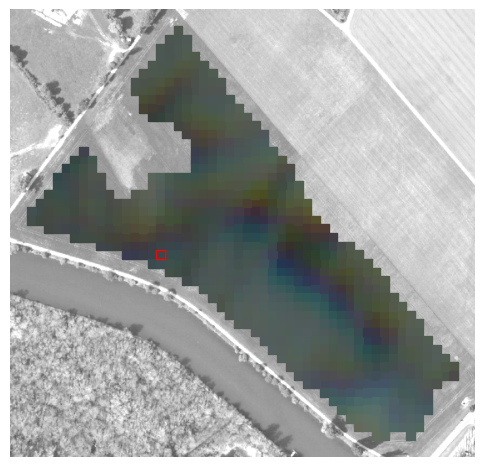
\includegraphics[width=\textwidth]{satelite/time_series_2021_P112/35_scl4_2021-06-03.png}
		\caption[2021-06-03\hspace*{0.1cm} SCL 4]%
		{{\small 2021-06-03\hspace*{0.1cm} SCL 4}}    
		\label{fig:satelite/time_series_2021_P112/35_scl4_2021-06-03.png}
	\end{subfigure}
	\hfill
	\begin{subfigure}[b]{0.31\textwidth}   
		\centering 
		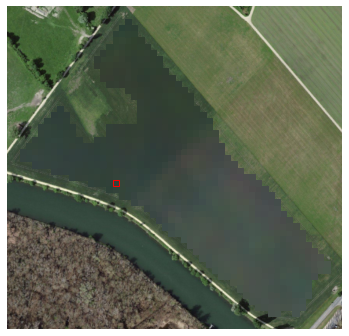
\includegraphics[width=\textwidth]{satelite/time_series_2021_P112/40_scl10_2021-06-28.png}
		\caption[2021-06-28\hspace*{0.1cm} SCL 10]%
		{\small 2021-06-28\hspace*{0.1cm} SCL 10}    
		\label{fig:satelite/time_series_2021_P112/40_scl10_2021-06-28.png}
	\end{subfigure}
	\hfill
	\begin{subfigure}[b]{0.31\textwidth}  
		\centering 
		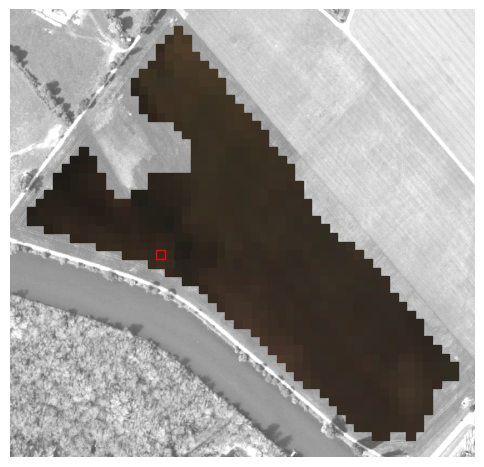
\includegraphics[width=\textwidth]{satelite/time_series_2021_P112/45_scl2_2021-07-23.png}
		\caption[2021-07-23\hspace*{0.1cm} SCL 2]%
		{{\small 2021-07-23\hspace*{0.1cm} SCL 2}}    
		\label{fig:satelite/time_series_2021_P112/45_scl2_2021-07-23.png}
	\end{subfigure}

	\vskip\baselineskip
	\begin{subfigure}[b]{0.7\textwidth}   
		\centering 
		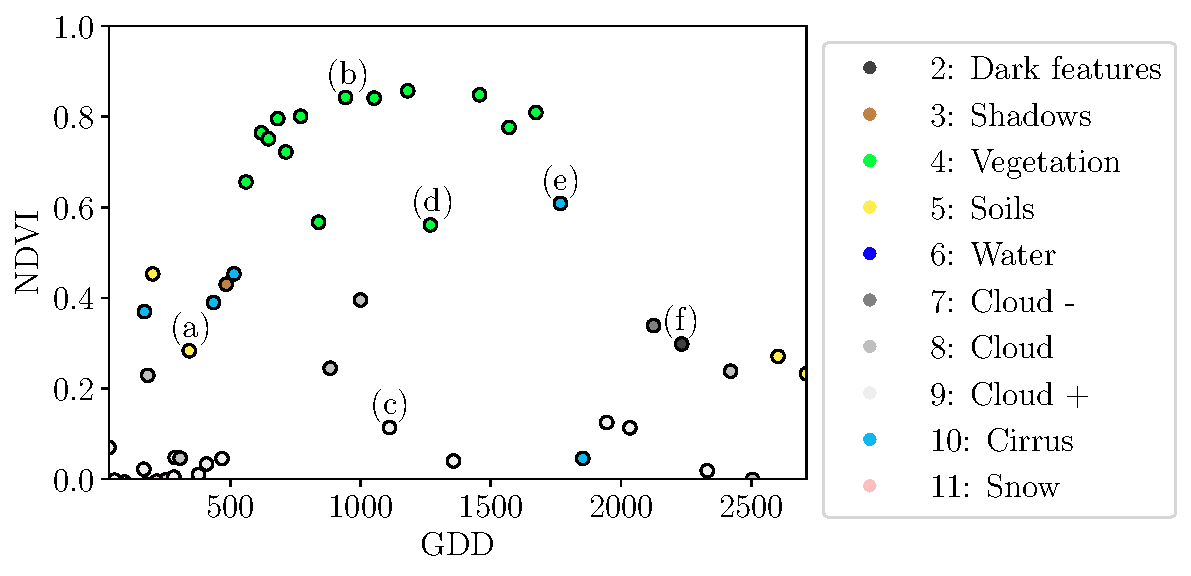
\includegraphics[width=\textwidth]{interpol/ndvi_ts_scl.pdf}
		\caption[Corresponding NDVI {TS}]%
		{{\small Corresponding NDVI {TS}}}    
		\label{fig:interpol/ndvi_ts_scl45_grey.pdf}
	\end{subfigure}
	\vspace{0.3cm}
	\caption[Satellite images of a field at selected times + NDVI TS]{Satellite images of a field at selected times with a static grayscale background for orientation. Moreover, the NDVI {TS} of the red-highlighted pixel is shown in (g) colored by the SCL labels.} 
	\label{fig:witzwil_selected_satellite_images}
\end{figure*}



			% Description of plot
			The figure ~\ref{fig:witzwil_selected_satellite_images} shows a selection of 6 satellite images of a field, which display our challenges. In February (image(a)), as expected, we see no vegetation but bare soil. At the beginning of May we observe a cloudless dark green field. In (c) it is obvious that we have no chance to get useful information when there is a heavy cloud cover. Figure (d) shows that the SCL classification is not reliable, since we evidently observe clouds. In (e) we see a pale green. This likely shimmers through cirrus clouds. 
			
			%% subfigures references:
			% (see. \ref{fig:satelite/time_series_2021_P112/15_scl5_2021-02-23.png})
			% (see. \ref{fig:satelite/time_series_2021_P112/30_scl4_2021-05-09.png})
			% (see. \ref{fig:satelite/time_series_2021_P112/33_scl9_2021-05-24.png})
			% (see. \ref{fig:satelite/time_series_2021_P112/35_scl4_2021-06-03.png})
			% (see. \ref{fig:satelite/time_series_2021_P112/40_scl10_2021-06-28.png})
			% (see. \ref{fig:satelite/time_series_2021_P112/45_scl2_2021-07-23.png})
		}
	}

	\subsection{Yieldmapping Data}{
		\label{sec:yieldmapping_data}
		The crop yield data were collected using a combine harvester. Equipped with GPS, the harvester drives over the fields and continuously estimates the crop density in $t/ha$ (see fig. \ref{fig:satelite/witzwil_2021_P112_yield_harvester_cropped}). 
		We take the data set derived from this in REF-Gregor-Perich, where error-prone measurement points (such as during an egen curve) were removed and then the yield map was rasterized using linear interpolation (cf. fig. \ref{fig:satelite/witzwil_2021_P112_yield_cropped.png}).    

		
		Comparing the manually weighted yield and the sum of estimated raster (per field per year) we note a discrepancy of about $10\%$ (cf. REF-gregor). Since the relative estimation error is rather constant and we do not aim to estimate the absolute yield we will not consider this deviation.
		\begin{figure}
			\centering
			\begin{subfigure}{.5\textwidth}
			  \centering
			  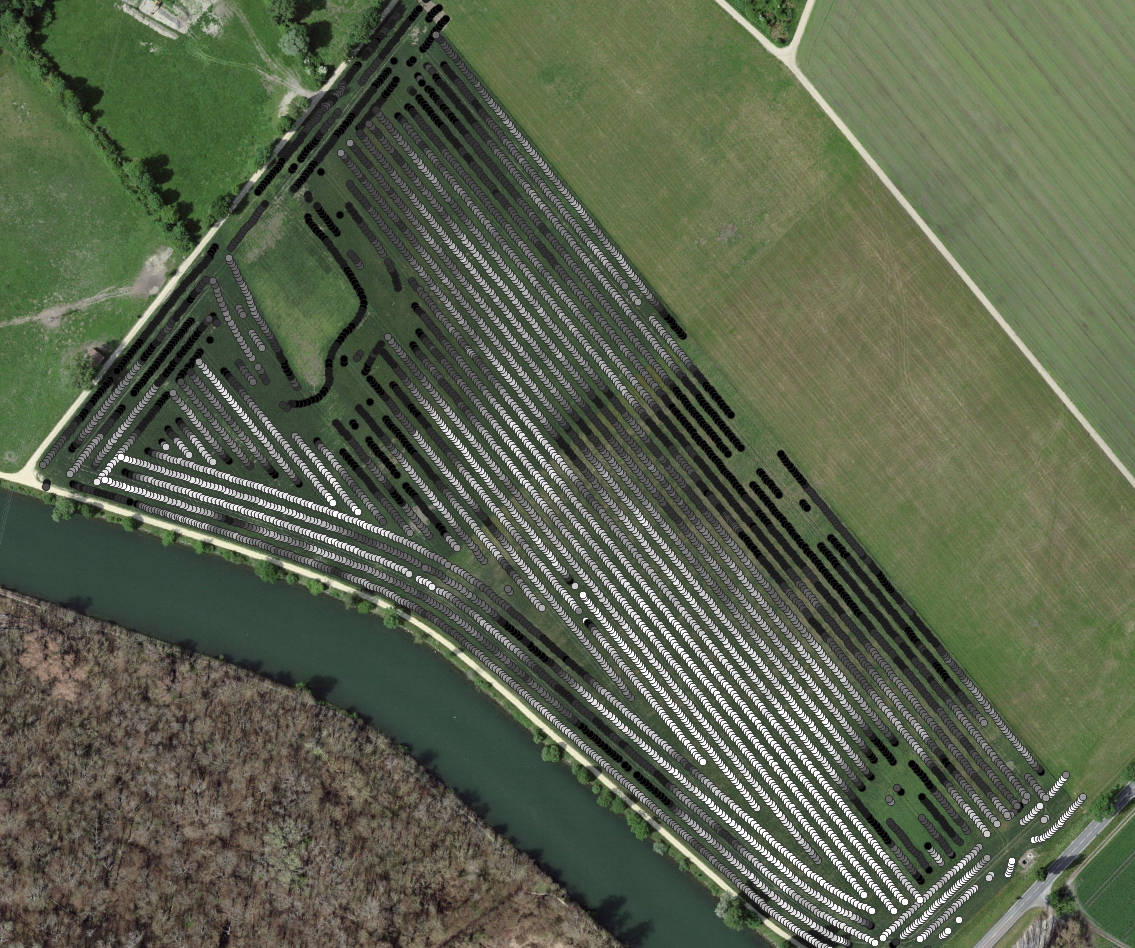
\includegraphics[height=.75\linewidth]{satelite/witzwil_2021_P112_yield_harvester_cropped.png}
			  \caption{obtained by a combine harvester (cleaned)}
			  \label{fig:satelite/witzwil_2021_P112_yield_harvester_cropped}
			\end{subfigure}%
			\begin{subfigure}{.5\textwidth}
				\centering
				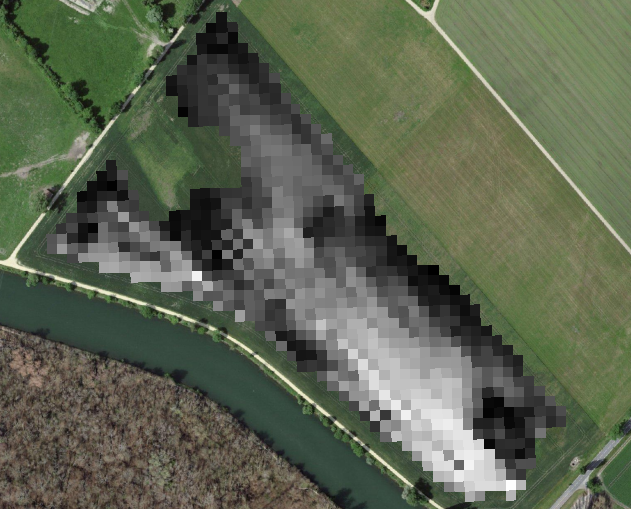
\includegraphics[height=.75\linewidth]{satelite/witzwil_2021_P112_yield_cropped.png}
			  \caption{rasterized to Sentinel 2 resolution.}
			  \label{fig:satelite/witzwil_2021_P112_yield_cropped.png}
			\end{subfigure}
			\caption{Crop yield density map of a field. Ranges from 0.1 t/ha (black) to 5.35 t/ha (white) }
			\label{fig:satelite_witzwil_yield}
		\end{figure}
	}


	\subsection{Gather Data}{
		\label{sec:gather_data_to_pixel}
		Before we join all the data, we define a few concepts.

		{% NDVI
			Using bands $B4$ and $B8$, we calculate the well-known Normalized Difference Vegetation Index (\textit{NDVI}) using the formula: (???REF nötig?)
			\begin{equation}
				NDVI = \frac{B8 - B4}{B8 + B4}
				\label{eq:ndvi}
			\end{equation}
			Note that we call the calculated values merely the \textit{observed NDVI}, as we must be aware of imprecisions due to clouds and shadows. 
		}

		{% GDD & DAS
			To define a timescale, we consider Days After Sowing (\textit{DAS}) and a transformed timescale, Growing Degree Days (\textit{GDD}) (\cite{mcmasterGrowingDegreedaysOne1997}). The latter are defined as the cumulative sum (since sowing) of temperature above a given base temperature $T_{base}$ \footnote{XXX For cereals we use $T_{base}=0$ }. Thus, the GGD for $n$ days after sowing will be equal to:
			\begin{equation}
				\label{eq:gdd}
				GDD_n := \sum_{i=0}^n \max(T_i - T_{base}, 0).
			\end{equation}
		} 

		Now we create a data set, which will contain all necessary information. Given that we have the spectral data at a $10m \times 10m$ resolution, we introduce the concept of a Pixel. A \textit{Pixel} $P$ is associated with a $10m \times 10m$ square defined by the S2 satellites and contains all relevant information for a season and this location. More precisely, $P$ is a collection of general information (like yield and coordinates) and all associated $P_t$ of a given season. Where $P_t$ represents a tuple of the spectral data for time $t$, the NDVI calculated from it, and the associated GDD. 
		We will call the resulting data set \textit{PIXELS} as it is the collection of all Pixels (over all seasons). 
		
		Finally we split PIXELS randomly into a train ($80\%$) and test  ($20\%$) set. 

	}

% \begin{my_pros_cons_table}{
%         \item 1
%         \item 2
%     }{
%         \item 1
%         \item 2
%     }
% \end{my_pros_cons_table}
\newcommand{\RobItPlot}{fitted to different (SCL45) NDVI {TS}. Iterations of a robustifying refit (as indicated in section~\ref{sec:loess_robustify}) are also displayed.}


\chapter{Interpolation} \label{sec:itpl}
	{% Roadmap
		The need for interpolating the NDVI {TS} was established in the precious chpater. In this chapter, we first specify a setting for the interpolation and categorize the {{IM}}s into those that make fundamental shape assumptions (parametric) and those that are more flexible (non-parametric). We give an introduction for each method with a compact definition, highlight adjustments or give remarks where appropriate, and point out strengths and weaknesses of each method. A brief overview of the considered {{IM}}s is provided in table~\ref{table:pros_cons_overview}.
		% In this section, we take a closer look at several {{IM}}s, which will be used to interpolate and smooth the NDVI {TS}, while considering only SCL45 in this chapter. First, we define the general setting and discuss a general approach to make the interpolation more robust (i.e., reduce the impact of outliers). Afterwards, we introduce and discuss each method.
		Afterwards, we extract a robustification strategy from one {{IM}} and generalize it, so we can use it for all methods that allow for a priori weighted observations. Finally, using LOOCV, we tune the parameters (where necessary) and get a first idea of the performance of each method.


	}
	{% pros & cons table
		\footnotesize
		\begin{table}[!ht]
	\centering
	\todo[inline]{add fourier  and fix order to match chapters}
	\caption[skip=10pt]{Summary of the studied interpolation methods containing important assumptions, advantages and disadvantages and whether the method supports weighted observations (w) and if the resulting interpolation is bounded w.r.t. a fixed interval (b).}
	\small
	\begin{tabular}{p{1.6cm}p{3.3cm}p{3.3cm}p{3.4cm}p{0.4cm}p{0.4cm}p{3cm}p{3cm}p{3cm}p{3cm}p{2.7cm}p{3cm}|}
		\toprule
		% \hline
		~                                                                                                                                                            &
		\textbf{Assumptions}                                                                                                                                         &
		\textbf{Advantages}                                                                                                                                                &
		\textbf{Disadvantages}                                                                                                                                                &
		\textbf{w}                                                                                                                                      &
		\textbf{b}                                                                                                                                        \\ \hline

		Savitzky-Golay filter                                                                                                                                        &
		\begin{cptitemize}
			\item[--]  High frequencies are noise (Low-Pass-Filter) \item[--]  Equidistant points \item[--]  Local polynomials
		\end{cptitemize}                                              &
		\begin{cptitemize} \item[--]  Computationally very fast                                                                   \end{cptitemize}                   &
		\begin{cptitemize} \item[--]  Cannot deal natively with missing data (need some interpolation)                              \end{cptitemize}                 &
		No                                                                                                                                                           &
		(Yes)                                                                                                                                                         \\ \hline%comment out?

		SG +~NDVI                                                                                                                                                    &
		\begin{cptitemize} \item[--]  Upper envelope \item[--]  Vegetation cannot grow faster than some slope                                \end{cptitemize}        &
		\begin{cptitemize} \item[--]  Biological knowledge                                                                            \end{cptitemize}               &
		\begin{cptitemize} \item[--]  Bad ``upper envelope'' since weights are not used for the estimation itself                    \end{cptitemize}               &
		(No)                                                                                                                                                         &
		(Yes)                                                                                                                                                         \\ \hline%comment out?

		LOESS                                                                                                                                                        &
		\begin{cptitemize} \item[--]  Local  polynomial with points closer to the estimated point are more important                  \end{cptitemize}               &
		\begin{cptitemize} \item[--]  Flexible \item[--]  Generalization of SG \item[--]  Weighting function makes intuitive sense                  \end{cptitemize} &
		\begin{cptitemize} \item[--]  Computationally expensive                                                                       \end{cptitemize}               &
		Yes                                                                                                                                                          &
		(Yes)                                                                                                                                                         \\ \hline%comment out?

		Smoothing Splines                                                                                                                                            &
		\begin{cptitemize} \item[--]  2cd derivative of function is integrable                                                        \end{cptitemize}               &
		\begin{cptitemize} \item[--]  Intuitive meaning of penalty \item[--]  General assumptions \item[--]  Flexible shape                         \end{cptitemize} &
		\begin{cptitemize} \item[--]  Unbounded                                                                                       \end{cptitemize}               &
		Yes                                                                                                                                                          &
		No                                                                                                                                                             \\ \hline%comment out?

		B-Splines (Smoothed)                                                                                                                                         &
		\begin{cptitemize} \item[--]  Function can be approximated by a linear combination of B-splines basis functions               \end{cptitemize}               &
		\begin{cptitemize} \item[--]  General assumption \item[--]  Flexible shape                                                            \end{cptitemize}        &
		\begin{cptitemize} \item[--]  Unbounded \item[--]  No intuitive meaning for smoothing                                                \end{cptitemize}        &
		Yes                                                                                                                                                            &
		No                                                                                                                                                             \\ \hline%comment out?

		% Penalized Regression Splines &
		% \begin{itemize}
		%     \item[--]  High
		%     \item[--]  Bs
		% \end{itemize} &
		% ~ &
		% ~ &
		% ~ &
		% ~ \\ \hline%comment out?

		% Whittaker                                                                                                                                                    &
		% % \parskip=0pt
		% % \begin{minipage}[t]{\linewidth}
		% % 	\begin{itemize}[nosep,after=\strut]
		% % 		\item[--] First
		% % 		\item[--] Second
		% % 	\end{itemize}
		% % \end{minipage}                                                               &
		% ~                                                                                                                                                            &
		% ~                                                                                                                                                            &
		% ~                                                                                                                                                            &
		% ~                                                                                                                                                              \\ \hline%comment out?

		(Gaussian) Kernel Smoothing                                                                                                                                  &
		\begin{cptitemize} \item[--]  Close points are related to each other via a kernel function \end{cptitemize}                                                                                                                                                            &
		\begin{cptitemize} \item[--]  Simple \item[--]  General assumptions                                                                  \end{cptitemize}        &
		\begin{cptitemize} \item[--]  Bandwidth: fails if there are big data-gaps                                                     \end{cptitemize}               &
		Yes                                                                                                                                                          &
		Yes                                                                                                                                                            \\ \hline%comment out?

		% Fourier                                                                                 &
		% ~                                                                                       &
		% ~                                                                                       &
		% ~                                                                                       &
		% ~                                                                                       &
		% ~                                                                                             \\ \hline%comment out?

		Double-Logistic                                                                                                                                              &
		\begin{cptitemize} \item[--]  Function first increases then decreases \item[--]  Ndvi has a minimal value                            \end{cptitemize}        &
		\begin{cptitemize} \item[--]  Good for evergreen plants (if snow masks NDVI) \item[--]  Upper envelope                                \end{cptitemize}        &
		\begin{cptitemize} \item[--]  Parameter estimation can go seriously wrong \item[--]  Strange behavior for long data-gaps             \end{cptitemize}        &
		Yes                                                                                                                                                          &
		(Yes)                                                                                                                                                         \\ \hline%comment out?

		Universal Kriging                                                                                                                                            &
		\begin{cptitemize} \item[--]  Function is a realization of a stationary Gaussian process                                      \end{cptitemize}               &
		\begin{cptitemize} \item[--]  Informative parameters \item[--]  Flexible                                                             \end{cptitemize}        &
		\begin{cptitemize} \item[--]  Regression to the mean \item[--]  Assumptions clearly not met                                          \end{cptitemize}        &
		Yes                                                                                                                                                          &
		(Yes)                                                                                                                                                         \\ %\hline%comment out?

		% methodname &
		% ~ &
		% ~ &
		% ~ &
		% ~ &
		% ~ \\ \hline%comment out?
		\bottomrule
	\end{tabular}
	\label{table:pros_cons_overview}
\end{table}

		\normalsize
	}



\section{Interpolation Setup}{\label{sec:itpl_setup}
	For now, we will only consider SCL45 observations since they are more reliable. Hence, data in the form of $\left(t_{i}, y_{i}\right)$ for $i=1, \ldots, n$ is given, where $t_i$ is the time in GDD and $y_i$ denotes the NDVI at $t_i$. We assume that it can be represented by
	$$
		y_{i}=m\left(t_{i}\right)+\varepsilon_{i},
	$$
	where $\varepsilon_i$ is some random noise and $m: \R \rightarrow \R$ is some (parametric or non-parametric) function. If we assume that $\varepsilon_{1}, \ldots, \varepsilon_{n}$ i.i.d. with $\mathbb{E}\left[\varepsilon_{i}\right]=0$ then 
	$$
		m(t)=\mathbb{E}[y \mid t]
	$$
	We will introduce parametric and non-parametric approaches to estimate $m$ in section~\ref{sec:itpl_parametric} and~\ref{sec:itpl_nonparametric}.
	Furthermore, in the subsequent, we denote $w\in \R^n$ as the vector of weights such that $w_i$ corresponds to the weight that $(t_i, y_i)$ should have in the interpolation. 
}



\todo[inline]{Paper zitieren wo eingeführt oder wo benutzt (falls einführung fast schon trivial)}

\section{Parametric Regression} 
	\label{sec:itpl_parametric}
	Parametric Curve estimation tries to fit a parametric function, such as, for example, a Gaussian function with parameters $\mu$ and $\sigma$, to a dataset. In the following, we introduce two parametric approaches.

	\subsection{Double Logistic (DL)}
		\label{sec:double_logistic}
		The Double Logistic smoothing as described in \cite{beckImprovedMonitoringVegetation2006} heavily relies on shape assumptions of the fitted curve (i.e. the NDVI time series). First, we assume that there  is a minimum NDVI level $y_{\min}$ in the winter (e.g. due to evergreen plants), which might be masked by snow. This can be estimated beforehand, taking several years into account. Second, we assume that the growth cycle can be divided into an increase and a decrease period, where the time series follows a logistic function. The maximum increase (or decrease) is observed at $t_0$ (or $t_1$) with a slope of $d_0$ (or $d_1$). The equation of the double-logistic fit is given by:
		\begin{equation*}
			y(t) = y_{\min} + \left(y_{\max}-y_{\min}\right)\left(\frac{1}{1+e^{-d_0(t-t_0)}}+\frac{1}{1+e^{-d_1(t-t_1)}}-1\right)
		\end{equation*}
		Where the five free parameters: $y_{\max}$, $d_0$, $d_1$, $t_0$, $t_1$ are initially estimated by least squares. Such fit can be seen in figure~\ref{fig:interpol/fourier_dl_comparison}.

		\subsubsection*{Robustification}
		Similar as for the SG (c.f. section~\ref{sec:Savitzky-Golay}) one can reestimate (only once) the parameters by giving less weight to the overestimated observations and more weight to the underestimated observations. For the details on the choice of the weights we refer to \cite{beckImprovedMonitoringVegetation2006}. We will not apply this reestimation but rather the robustification introduced later in section \ref{sec:loess_robustify}.

		\begin{my_pros_cons_table}{
				\item Incorporates subject specific knowledge in the case of evergreen plants covered in snow.
				\item Optimized parameters have an intuitive meaning.
			}{
				\item Strong shape assumptions on the NDVI curve.
				\item Parameter optimization might go wrong. This can be mitigated to some extent to provide bounds for the parameters
				\item Strange behavior in regions with little observations. (c.f. figure~\ref{fig:interpol/fourier_dl_comparison})
			}
		\end{my_pros_cons_table}


	\subsection{Fourier Series (FS)}
		\label{sec:fourier_approx}
		\cite{stockliEuropeanPlantPhenology2004} approximates the NDVI curve using a second order FS:
		$$
			\operatorname{NDVI}(t)=\sum_{j=0}^{2} a_{j} \times \cos \left(j \times \Phi_{t}\right)+b_{j} \times \sin \left(j \times \Phi_{t}  \right)
		$$
		where $\Phi=2 \pi \times(t-1) / n$. Thus, we periodical behavior. If we would set the period to match one year this would coinced with the notion that plans grow every year. 
		Analogous to section~\ref{sec:double_logistic} we fit it to the data by least squares.
		Example fits can be seen in figure \ref{fig:interpol/fourier_dl_comparison}


		% \cite{beckImprovedMonitoringVegetation2006} shows in their lag-plots a heavy autocorrelation of resiudals

		\begin{my_pros_cons_table}{
				\item Assumption of periodicity can be helpful if we are modelling multiyear grow cycles
				\item Flexible curve shape
			}{
				\item Bad behavior in regions with little data (c.f. figure~\ref{fig:interpol/fourier_dl_comparison})
				\item Hard to interpret estimated parameters
				\item Parameter estimation can go wrong. Introducing bounds can help.
			}
		\end{my_pros_cons_table}

		\begin{my_figure}[h]{width=1\textwidth}{interpol/fourier_dl_comparison}
			\caption{Here we observe the possibilities of a precise fit for the two parametric methods but notice also some misbehavior}
			\label{fig:interpol/fourier_dl_comparison}
		\end{my_figure}

	\subsection{Optimization Issues}\label{sec:itpl_param_optimizationissues}
		We shall mention some optimization issues we countered during implementation. Since we aim to minimize the residual sum of squares over 5 (or 6) parameters, we try to solve a non-convex optimization problem. Thus, the algorithm\footnote{We used the python function \texttt{scipy.optimize.curve\_fit}.} either struggles to find the global minimum or fails to converge. This was fixed by providing for each parameter reasonable initial values and generous bounds (that match our experience).

\section{Non-Parametric Regression}
	\label{sec:itpl_nonparametric}
	In non-parametric curve estimation, the curve does no longer have to be fully determined by parameters, but we allow it to flexibly approximate the data. Note that we do not exclude the use of tuning-parameters.

	\subsection{Kernel Regression: Nadaraya-Watson (NW)}
		\label{sec:Kernel}
		As described in section \ref{sec:itpl_setup}, we aim to estimate
		\begin{equation}
			\label{eq:nadaraya}
			\mathbb{E}[Y \mid T=t]
			= \int_{\R} y f_{Y \mid T}(y \mid t) d y
			=\frac{\int_{\R} y f_{T, Y}(t, y) d y}{f_{T}(t)},
		\end{equation}
		where $f_{Y \mid T}, f_{T, Y}, f_{T}$ denote the conditional, joint and marginal densities.
		This can be done with a kernel $K$:
		\begin{equation}
			\hat{f}_{T}(t)=\frac{\sum_{i=1}^{n} K\left(\frac{t-t_{i}}{h}\right)}{n h}, \quad \hat{f}_{T, Y}(t, y)=\frac{\sum_{i=1}^{n} K\left(\frac{t-t_{i}}{h}\right) K\left(\frac{y-Y_{i}}{h}\right)}{n h^{2}},
			\label{eq:kernel_with_bandwidt}
		\end{equation}
		where $h$, the bandwidth, symbolizes the windowsize of to consider. By using the above function in equation \eqref{eq:nadaraya} we arrive at the NW kernel estimator:
		$$\hat{m}(t)=\frac{\sum_{i=1}^{n} K\left(\left(t-t_{i}\right) / h\right) Y_{i}}{\sum_{i=1}^{n} K\left(\left(t-t_{i}\right) / h\right)}$$

		Common choices for the kernel are the normal function or a uniform function (also called `bot' function). 
		\subsubsection*{Choose Bandwidth}
		Note that we still need to choose the bandwidth of the function. This can be done with the help of LOOCV while optimizing the RMSE. For non-equidistant data we refere to \cite{brockmannLocallyAdaptiveBandwidth1993} where a local adaptive bandwidth selection is presented.

		\begin{my_pros_cons_table}{
				\item fletible due to different possible kernels
				\item can be assigned degrees of freedom (trace of the hat-matrit)
				\item estimation of the noise variance $\hat \sigma_\varepsilon^2$ (REF c.f. CompStat 3.2.2)
			}{
				\item if the $t \mapsto K(t)$ is not continuous, $\hat m $ isn't either
				\item choice of bandwidth, especially if $t_i$ are not equidistant.
			}
		\end{my_pros_cons_table}


	\subsection{Universal Kriging (UK)}
		\label{sec:Kriging}

		UK as described in \cite{diggleGaussianModelsGeostatistical2007} was developed in geostatistics to deal with autocorrelation of the response variable at locations that are spatially close. By applying the notion that two spectral indices that are timewise close should also take similar values, we justify the application of UK. In the end, we would like to fit a smooth Gaussian process to the data.

		% definition (gaussian process)
		A Gaussian Process $\{S(t) : t\in \mathbb R\} $ is a stochastic process if $(S(t_1),\dots,S(t_k))$ has a multivariate Gaussian distribution for every collection of times ${t_1, \dots , t_k}$. $S$ can be fully characterized by the mean $\mu(t):=E[S(t)]$ and its covariance function $\gamma\left(t, t^{\prime}\right):=\operatorname{Cov}\left(S(t), S\left(t^{\prime}\right)\right)$. 
		% stationarity assumtpion
		Furthermore, we will assume the Gaussian process to be stationary. That is for $\mu(t)$ to be constant in $t$ and $\gamma(t,t')$ to depend only on $h=t-t'$. Thus, we will write in the following only $\gamma(h)$.\footnote{Note that the process is also \textit{isotropic} (i.e. $\gamma(h)=\gamma(\|h\|$) since we are in a one-dimensional setting and the covariance is symmetric.}

		% variogram
		Now, we need to make some assumption on the covariance function. For this we introduce the variogram of a Gaussian process as
		$$V(h):=V\left(t, t+h\right):=\frac{1}{2} \operatorname{Var}\left(S(t)-S(t+h)\right)\\ %align XXX
			=\gamma(0) + \gamma(t)
		$$
		and define $\gamma$ via the above equation by choosing the Gaussian Variogram defined by
		$$V(h) = p \cdot\left(1-e^{-\frac{h^{2}}{\left(\frac{4}{7} r\right)^{2}}}\right)+n.$$
		Here $h$ denotes the distance, $n$ is the nugget, $r$ is the range and $p$ is the partial sill. The influence of the parameters is visualized in figure~\ref{fig:interpol/kriging_gauss_variogram}.\footnote{Strictly speaking we use a scaled version of the variogram. Thus, only the ratio of $p/n$ matters.}

			\begin{my_figure}[h]{width=0.7\textwidth}{interpol/kriging_gauss_variogram}
				\caption{Gaussian Variogram with nugget=1, partial sill=3, range=55}
				\label{fig:interpol/kriging_gauss_variogram}
			\end{my_figure}

			\begin{my_figure}{width=1\textwidth}{interpol/kriging_parameter}
				\caption{On the left, we see how the interpolation change if we increase the nugget and the range parameter. On the right, we compare two UK interpolations, where one takes parameters by numerically maximizing the (which results in a very small nugget) and the other takes the median of many such numerical optimizations.}
				\label{fig:kriging_parameters}
			\end{my_figure}

		Finally, we consider a one-dimensional Gaussian process $G_\gamma$ with variogram $\gamma$ and tune the variogram parameters using matimum likelihood\footnote{As illustrated in figure~\ref{fig:kriging_parameters} matimum likelihood estimation can lead to overfitting. Thus, we will in practice sample several such optimized parameters and use their median in the end.}. Let $z$ be a vector with the new values to ettrapolate, then we can determine the values $m(z) = \mathbb{E}\left[G_\gamma(z) | (t,y)\right]$ using Bayes rule\footnote{Bayes rule generally claims that for two random variables $A$ and $B$ we have that $P(A|B) = P(B|A) / P(B)$}. For an etample fit, we refer to figure~\ref{fig:kriging_parameters}. 

		\subsubsection*{Violated Assumption}
			Since we observe a clear pattern of a growth period in spring and harvest in the end of summer, we have to admit that our stationarity assumtpion with the constant mean is structurally violated. This is also the reason why we observe (for every variogram parameter) a tendency to the mean, as indicated in figure~\ref{fig:kriging_parameters}.

		\begin{my_pros_cons_table}{
				\item It is a well-studied method.
				\item Variogram parameters have an intuitive meaning.
				\item Flexible covariance structure.
			}{
				\item Regression to the mean.
				\item Violated assumption of constant mean and constant variance. Thus, the NDVI is not a stationary process.
				\item Pure maximum likelihood can result in overfitting.
			}
		\end{my_pros_cons_table}


	\subsection{Savitzky-Golay Filter (SG)}
		\label{sec:Savitzky-Golay}
		The SG, introduced in \cite{savitzkySmoothingDifferentiationData1964} is a technique in signal processing and can be used to filter out high frequencies (low-pass filter) \citep{schaferWhatSavitzkyGolayFilter2011}. Furthermore, it can also be used for smoothing by filtering high frequency noise while keeping the low frequency signal.

		First, we choose a window size $m$. Then, for each point, $j \in \{m, m+1, \dots, n-m\}$ we fit a polynomial of degree $k$ by:
		$$\hat y_j=\min_{p\in P_k}\sum_{i=-m}^{m}(p (t_{j+i})-y_{i+j})^{2},$$
		where $P_k$ denotes the Polynomials of degree $k$ over $\R$.
		For equidistant points this can efficiently be calculated by
		$$
			\hat y_{j}=\sum_{i=-m}^{m} c_{i} y_{j+i},
		$$
		where the $c_i$ are only dependent on the $m$ and $k$ and are tabulated in the original paper.

		\cite{chenSimpleMethodReconstructing2004a} developed a `robust' interpolation method for the NDVI based on the SG. 
		The method is based on the assumption that due to atmospheric effects the observed NDVI tends to be underestimated and that it cannot increase too quickly. The latter is argued by the biological impossibility of such fast vegetation changes. Their proposed algorithm is:\todo{figure / tabelle / pseudocode anstatt aufzählung}
			\begin{enumerate}
				\item Remove non-SCL45 points.
				\item Remove points that would indicate an increase greater than 0.4 within 20 days.
				\item Linearly interpolate to obtain an equidistant time series $X^0$.
				\item Apply the SG to obtain a new time series $X^1$.
				\item Update $X^1$ by applying again a SG. Repeat this until $w^T |X^1-X^0|$ stops decreasing, where w is a weight vector with $w_i = \min\left(1, 1 - \frac{X^1_i-X^0_i}{\max_i\|X^1_i-X^0_i\|}\right)$. This reduces the penalty introduced by outliers\footnote{Here we call a point $i$ an outlier if $X^0_i<X^1_i$.} and by repeating this step we approach the ``upper NDVI envelope''.
			\end{enumerate}

		\subsubsection*{Extension: Spatial-Temporal SG}
			One notable adaptation of the SG is the presented by \cite{caoSimpleMethodImprove2018b}. The key difference is the additional assumption of the cloud cover being discontinuous and that we can improve by looking at adjacent pixels\footnote{Here, we say that a pixel is adjacent if it is the same pixel but from a different year (keeping the same day of the year) or (if not enough of such temporal-adjacent pixel are found) it is spatially adjacent}. Because we are working with rather high resolution satellite data, and we need the variance in the predictors, we will waive this extension.

		\begin{my_pros_cons_table}{
				\item Popular technique in signal processing.
				\item Efficient calculation for equidistant points.
				\item Upper envelope matches intuition for the NDVI. Therefore, it is robust against outliers with small values.
			}{
				\item No natural way of how to estimate points that are not in the data.
				\item Not generalizable to other spectral indices.
				\item Linear interpolation to account for missing data might be not appropriate.
				\item No smooth interpolation between two measurements.
			}
		\end{my_pros_cons_table}


	\subsection{Locally Weighted Regression (LOESS)}
		\label{sec:loess}
		% Introduced by : \cite{clevelandRobustLocallyWeighted1979}
		% implemented here \cite{cappellariATLAS3DProjectXX2013}

		The LOESS introduced by \cite{clevelandRobustLocallyWeighted1979} can be understood as a generalization of the SG (c.f. sec.~\ref{sec:Savitzky-Golay}).

		Given a proportion $\alpha \in (0,1]$, we estimate each $y_i$ separately by fitting a polynomial of order $d$ by weighted least squares. The weights are (usually) defined by
		$$w_i(t_j)=\begin{cases}
				\left(1-\left(\frac{|t_j-t_i|}{h_i}\right)^{3}\right)^{3}, & \text{for } |t_j-t_i|<h_i           \\
				0,                                                   & \text{for } |t_j-t_i| \geqslant h_i
			\end{cases} ,$$
		where $h_i$ is the minimal distance such that $\lceil \alpha n\rceil$ observations are in the ball $B_{h_i}(t_i)$.\footnote{\label{footnote:LOESS}If too many weights are set to zero, we might end up considering not enough observations and thus get a singular design-matrit (for the least squares estimation). Therefore, we substitute $h_i$ with $1.01 h_i$, so that the observation on the boundary of $B_{h_i}(t_i)$ does not get completely ignored. But we also have to assure that $\alpha$ is big enough.} So for each $y_i$ we only consider a proportion $\alpha$ of the observations.

		\subsubsection{Differences between the Robust LOESS and the SG?}
		The LOESS smoother takes a fraction of points instead of a fixed number and therefore automatically adapts to the size of the data we wish to interpolate. However, we run into the danger of considering too little observations, since the estimation breaks down if $\lceil \alpha n\rceil < d+1$.\footnoteref{footnote:LOESS}
		Furthermore, LOESS gives less weight to points further away. This yields a "smoother" estimate, since when we slide the window (e.g. for estimating the next value) an influential point at the border does not suddenly get zero weight from being weighted equally before.
		Finally, the LOESS also can be used for non-equidistant data and allows for arbitrary interpolation.

		\begin{my_pros_cons_table}{
				\item Flexible generalization of SG
				\item arbitrary interpolation possible
				\item Intuitive parameters
			}{
				\item The nature of local regression might lead to surprising estimates (no smoothness guarantees for the second derivative)
			}
		\end{my_pros_cons_table}


	\subsection{B-Splines (BS)}
		\label{sec:B}
		BS as discussed in \cite{lycheSplineMethods2005} are piecewise cubic polynomials defined by 
		$$
			S(t)=\sum_{j=0}^{n-1} c_{j} B_{j, k ; t}(t),
		$$
		where $B$ are basis functions and recursively defined by:
		
		\begin{equation}
				B_{i, 0}(z)=1, \text { if } t_{i} \leq z<t_{i+1}, \text { otherwise } 0 \\
		\end{equation}
		\begin{equation}
			B_{i, k}(z)=\frac{z-t_{i}}{t_{i+k}-t_{i}} B_{i, k-1}(z)+\frac{t_{i+k+1}-z}{t_{i+k+1}-t_{i+1}} B_{i+1, k-1}(z).
		\end{equation}
		
		Assuming that all $t_i$ are distinct, this yields an interpolation that fits the data perfectly. To reduce the amount of overfitting and increase the smoothness, we relax the constraint that we have to perfectly interpolate. Thus, we use the minimum number of basis functions\footnote{So we do not require one basis function for each neighboring pair of knots. SciPy uses FITPACK and DFITPACK, the documentation suggests that smoothness is achieved by reducing the number of knots used} such that:
		$$\sum_{i=1}^n(w_i (y_i - \hat y_i))^2 \leq s$$

		\begin{my_pros_cons_table}{
				\item can be assigned degrees of freedom
				\item extendable to "smooth" version
				\item performs also well if points are not equidistant
			}{
				\item smoothing process does not translate well to a interpretation (unlike SS)
				\item choice of smoothing parameter $s$
			}
		\end{my_pros_cons_table}


	\subsection{Smoothing Splines (SS)}
		\label{sec:Natural_SS}
		Let $\mathcal F$ be the Sobolev space (the space of functions of which the second derivative is integrable). Then the unique\footnote{Strictly speaking it is only unique for $\lambda > 0$} minimizer
		\begin{equation}
			\label{eq:ss}
			\hat m :=\argmin_{f \in \mathcal F} \sum_{i=1}^{n}w_i\left(y_{i}-{f}\left(t_{i}\right)\right)^{2}+\lambda \int {f}^{\prime \prime}(t)^{2} dt
		\end{equation}
			
		is a % natural\footnote{It is called natural since it is affine outside the data range ($\forall t\notin [t_1, t_n]:\hat m''(t) = 0$)} 
		cubic spline (i.e. a piecewise cubic polynomial function).
		The objective function ensures that we decrease the curvature while keeping the RMSE low.

		\subsubsection{XXX Whittaker}

		\begin{my_pros_cons_table}{
				\item Can be assigned degrees of freedom (trace of the hat-matrix).
				\item Efficient estimation (closed form solution).
				\item Intuitive penalty (we don't want the function to be too ``wobbly'' --- change slopes).
				\item Also performs well if points are not equidistant.
				\item Fixes the Runge's phenomenon (fluctuation of high degree polynomial interpolation).
			}{
				\item The tuning parameter $\lambda$ must be chosen. This can be done via cross validation and optimizing a score function (e.g. the RMSE). 
			}
		\end{my_pros_cons_table}


	% \subsection{XXX Whittaker Smoother}

	% \label{sec:whittaker}
	% XXX
	% from [HERE](https://eigenvector.com/wp-content/uploads/2020/01/WhittakerSmoother.pdf):  
	%     The Whittaker Smoother: Eiler's paper[1] introduces the following objective function
	%     $$
	%     O(\mathbf{z})=(\mathbf{y}-\mathbf{z})^{\mathrm{T}} \mathbf{W}_{0}(\mathbf{y}-\mathbf{z})+\lambda_{\mathrm{s}} \mathbf{z}^{\mathrm{T}} \mathbf{D}_{\mathrm{s}}^{\mathrm{T}} \mathbf{D}_{\mathrm{s}} \mathbf{z}
	%     $$
	%     where $\mathbf{y}$ is a $N \times 1$ vector of measured data, $\mathbf{z}$ is smooth curve to be fit to the data, $\mathbf{W}_{0}$ is a diagonal matrix of weights (typically $0 \leq w_{0, n} \leq 1$ for $n=1, \ldots, N, \mathbf{D}_{\mathrm{s}}$ is a second derivative operator (e.g., $\mathbf{D}_{\mathrm{s}} \mathbf{z}$ is the second derivative of $\mathbf{z}$ ) and $\lambda_{\mathrm{s}}$ is a scalar penalty on the smoothing term. When data are missing, the corresponding weight, $w_{0, n}$, can be set to zero. Once that $\mathbf{W}_{0}$ and $\lambda_{\mathrm{s}}$ are given (set by default or provided by the user) the corresponding estimate of $\mathbf{z}$ is given by
	%     $$
	%     \hat{\mathbf{z}}=\left(\mathbf{W}_{0}+\lambda_{\mathrm{s}} \mathbf{D}_{\mathrm{s}}^{\mathrm{T}} \mathbf{D}_{\mathrm{s}}\right)^{-1} \mathbf{W}_{0} \mathbf{y}
	%     $$
	%     For example, an optical emission (OES) spectrum is plotted Figure 1 along with two smoothed versions shown for $\mathbf{W}_{0}=\mathbf{I}$ and $\lambda_{\mathrm{s}}=0.1$ (low smoothing) and $\lambda_{\mathrm{s}}=10$ (stronger smoothing).   
	% **Original paper states use of the first derivative**  
	% --> second derivative is very similar to SS
	% \begin{my_pros_cons_table}{
	%     \item 1
	%     \item 2
	%   }{
	%     \item 1
	%     \item 2
	%   }
	% \end{my_pros_cons_table}



% \subsection{Other Methods to study:}
% From introduction of \cite{chenSimpleMethodReconstructing2004a}:\\
% (1) threshold-
% based methods, such as the best index slope extraction
% algorithm (BISE) (Viovy et al., 1992); (2) Fourier-based
% fitting methods (Cihlar, 1996; Roerink et al., 2000; Sellers
% et al., 1994); and (3) asymmetric function fitting methods
% such as the asymmetric Gaussian function fitting approach
% (Jonsson Eklundh, 2002) and the weighted least-squares
% linear regression approach (Swets et al., 1999).

\section{Tuning Parameter Estimation}{ \label{sec:itpl_param_est}
	Many of the {{IM}}s introduced in section~\ref{sec:itpl_parametric} and~\ref{sec:itpl_nonparametric} include a free parameter. To determine this parameter for a specific {{IM}}, we will estimate the absolute residuals using OOB estimation and then optimize the parameter using a score function. We clarify the procedure step by step:	
	\begin{Nenumerate}
		\item Construct a set $\Lambda$ of candidate parameters that generously covers the parameter space.
		% \item Consider $\mathcal{P}$, a set of Pixels.
		% \item For each parameter $\lambda \in \Lambda$ consider the individual pixels and the LOOCV\footnote{For a definition of the leave-one-out-cross-validation we refer to section~\ref{sec:OOB_LOOCV}.} estimator for the specific NDVI {{IM}} for all Pixels in $\mathcal{P}$ simulatnously. 
		% \item Determine $\lambda_{optimal} = \argmin_{\lambda\in\lambda}q_{90}(R_\lambda)$, where we describe the 90\% quantile with $q_{90}$.
		\item Consider the vector $z:=(y_1^{(1)},\dots,y_{n_1}^{(1)},y_1^{(2)},\dots,y_{n_2}^{(2)},\dots,y_1^{(m)},\dots,y_{n_m}^{(m)},)$ of all NDVI TS for all $m$ pixels.
		\item Consider its LOOCV estimator $\hat z_\lambda$ using the specific IM and the parameter $\lambda$ for each pixel individually.
		\item Determine $\lambda_{optimal} = \argmin_{\lambda\in\lambda}\operatorname{QAR}^{90}(\hat z_\lambda)$
	\end{Nenumerate}

	\begin{my_figure}[h]{width=1\textwidth}{interpol/statistics_SS_param_optim}
		\caption[Smoothing splines optimized by minimizing the given quantile of the absolute leave-one-out residuals]{Smoothing splines fit with smoothing parameter optimized by minimizing the LOOCV QAR. Note that the larger the considered quantile is, the more the curvature of the resulting curve decreases.}
		\label{fig:interpol/statistics_SS_param_optim}
	\end{my_figure}

	We choose $\operatorname{QAR}^{90}$ as our optimization function because we want to allow 10\% of outliers (contaminated points) but also aim for an accurate fit in 90\% of the cases.  
	
	Figure~\ref{fig:interpol/statistics_SS_param_optim} exemplifies the effect of the chosen quantile in the optimization function (QAR\textsuperscript{x}). To summarize, we may say that the higher the quantile, the stronger the smoothing. 
}


\section{Robustification}{
	\label{sec:loess_robustify}
	{ % Intro
		Now we discuss a general approach of how to make an interpolation more robust against outliers. The main idea is to give less weight to observations that have high residuals after the initial (or if we reiterate, the previous) fit.

		Even though the procedure is taken from the robust version of the LOESS smoother (cf. section~\ref{sec:loess} and \cite{clevelandRobustLocallyWeighted1979}), we can apply it to every {{IM}} that allows for prior weighting of observations.
	}
	
	{	
		After an initial fit, we calculate the residuals $r_i := y_i - \hat y_i$ and obtain $\tilde r_i$ by scaling with the median of the absolute residuals: 
		\begin{equation}
			\tilde r_i := \frac{r_i}{6\operatorname{med}\left(|r_1|,\dots,|r_n|\right)}
		\end{equation}
		Next, we compute new weights by
		\begin{equation}
			w_i^\text{new}:=w_i^\text{old} \begin{cases}
				\left(1-\tilde r_i^{2}\right)^{2}, & \text{if } |\tilde r_i|<1 \\
				0,                        & \text{else }
			\end{cases};\quad
			\label{eq:bisquare}
		\end{equation}
		Using the new weights, we can re-interpolate. This reweighting can be iterated for several steps or till the change of the values is smaller than some tolerance.

	% Old more complicated version
		% Before we describe the procedure, we define a function that will determine the weight given to each observation, such that observations with large-scaled residuals will have less weight. That is the bisquare function B:
		% 	$$
		% 		B(x):=\begin{cases}
		% 			\left(1-x^{2}\right)^{2}, & \text{if } |x|<1 \\
		% 			0,                        & \text{else }
		% 		\end{cases}
		% 	$$ 
		% 	Now, we do something similar to what is done in iteratively reweighted least squares. After an initial interpolation, update the weights of each observation with
		% 	\begin{equation}
		% 		w_i^\text{new}:=w_i^\text{old} \operatorname{B}\left(     \right);\quad
		% 		r_i := y_i - \hat y_i
		% 		\label{eq:bisquare}
		% 	\end{equation}
		% 	and interpolate again using the new weights. We can iterate this reweighting and stop after several steps or when the change of the values is smaller than some tolerance.
	}

	Note that this procedure is indeed robust since we use the median for the normalization which has a breakdown point\footnote{Intuitively, the breakdown point denotes the fraction of observations a `vicious' player can replace without breaking the estimator. For example, the median has a breakdown point of $50 \%$.} of $50 \%$.\footnote{The breakdown point relates only to outliers in the $y$ values. Note that we do not require the {{IM}}s to be robust, since the residual for an outlier will  still be larger than for non-outliers and thus will be down weighted more and more in each iteration (because for the next iteration the residual of the outlier will be even larger, since we gave less weight to it).}
	\subsection{Our Adjustment:}{
		During the iterations or when supplying prior weights, low-weighted observations can corrupt our estimation of scale (the median of absolute residuals). Thus, we introduce the weighted median as
		$$
			\med_\text{weighted}(r,w) := \argmin_{\lambda \in \R} \sum_{i=1}^n |r_iw_i -\lambda|
		$$
		for $r,w\in \R^n$. 
	}
	\subsection{Examples and Conclusions}{		
		Examples of the first four iterative fits using SS and LOESS are shown in figure~\ref{fig:interpol/2x3_SS_robust} and~\ref{fig:interpol/2x3_loess_robust} for six pixels. For the analogous figures of BS and DL we refere to the appendix~\ref{fig:interpol/2x3_B-Splines_robust} and~\ref{fig:interpol/2x3_DL_robust}.
		Indeed, we observe how the interpolated {TS} is less affected by outliers after each iteration. We notice the biggest difference in the first iteration. Furthermore, in the plot at the bottom left we see how the interpolation `escapes' from the right endpoint with each successive iteration, even though our intuition does not necessarily identify this point as an outlier. Therefore, in the following, we will always stop after one iteration.

		\begin{my_figure}[h]{width=1\textwidth}{interpol/2x3_SS_robust}
			\caption[Smoothing splines robustification.]{Smoothing splines \RobItPlot}
			\label{fig:interpol/2x3_SS_robust}
		\end{my_figure}
		\begin{my_figure}[h]{width=1\textwidth}{interpol/2x3_loess_robust}
			\caption[The LOESS smoother robustification.]{The LOESS smoother \RobItPlot}
			\label{fig:interpol/2x3_loess_robust}
		\end{my_figure}
	} 
	
	\subsection{Upper Envelope Approach}
		If we artificially increase the negative residuals in~\refeq{eq:bisquare} (e.g.,  by multiplying with 2), the corresponding points will get less weight in the next iteration. This allows us to create an interpolation that resembles an upper envelope. Intuitively, this upper envelope can be thought of as a sheet that is laid on top of the points.
			
		This approach is based on the premise that we tend to underestimate the NDVI \citep{caoSimpleMethodImprove2018b}. Since we want to develop a general method that is in principle not related to the NDVI, we will not pursue this approach further.	
}
\section{Performance Assessment}{\label{sec:itpl_perfomance_assessment}
	Next, we will benchmark the in section~\ref{sec:itpl_preselection} preselected {{IM}}s with and without robustification. For this, we will use the same technique as we did for the parameter determination in section~\ref{sec:itpl_param_est}. On $B_\lambda$ we apply the score functions from section~\ref{sec:scorefun}.  

	The results are presented in section~\ref{sec:results_itpl} and are discussed in section~\ref{sec:discussion_itpl}. The double logistic turns out to be the best convincing parametric method, and from the non-parametric methods we choose the SS.
}



\chapter{NDVI Correction}



\begin{my_figure}[ht]{width=0.75\textwidth}{ndvi_corr/residuals_scl_classes}
    \caption{XXX caption XXX}
    \label{fig:ndvi_corr/residuals_scl_classes}
\end{my_figure}


\begin{my_figure}[h]{width=1\textwidth}{ndvi_corr/scl_residuals_scatter}
    \caption{XXX caption XXX}
    \label{fig:ndvi_corr/scl_residuals_scatter}
\end{my_figure}

\chapter{Results}\label{sec:results}

\section{Goodness of Fit for Selected {{IM}}s}{
	\label{sec:results_itpl}
	The benchmarks of the in section~\ref{sec:itpl_preselection} selected {{IM}}s (considering only SCL45 observations) with respect to various score functions are displayed in table~\ref{tab:cv-statistics_itpl-methods}. The score functions summarize the absolute values of the LOOCV residuals (the smaller, the better). For each of the 5 selected {{IM}}s, we consider the basic and the robustified (see section~\ref{sec:loess_robustify}) version.

	\begin{table}[h]
		\begin{center}
			\caption[Goodness of fit for {{IM}}s  measured with score functions.]{Comparing the goodness of fit for selected {{IM}}s --- measured with score functions (see section~\ref{sec:scorefun}) that take the LOOCV residuals as input. Colored row-wise.}
			\scriptsize
			\begin{tabular}{lrrrrrrrrrr}
\toprule
 & ss & loess & dl & bspl & fourier & ss rob & loess rob & dl rob & bspl rob & fourier rob \\
\midrule
rmse & {\cellcolor[HTML]{EEEEEE}} \color[HTML]{000000} 0.063 & {\cellcolor[HTML]{F1F1F1}} \color[HTML]{000000} 0.061 & {\cellcolor[HTML]{F1F1F1}} \color[HTML]{000000} 0.061 & {\cellcolor[HTML]{DCDCDC}} \color[HTML]{000000} 0.074 & {\cellcolor[HTML]{DADADA}} \color[HTML]{000000} 0.075 & {\cellcolor[HTML]{E2E2E2}} \color[HTML]{000000} 0.070 & {\cellcolor[HTML]{EBEBEB}} \color[HTML]{000000} 0.065 & {\cellcolor[HTML]{EBEBEB}} \color[HTML]{000000} 0.065 & {\cellcolor[HTML]{D3D3D3}} \color[HTML]{000000} 0.079 & {\cellcolor[HTML]{000000}} \color[HTML]{F1F1F1} 0.208 \\
qtile50 & {\cellcolor[HTML]{747474}} \color[HTML]{F1F1F1} 0.036 & {\cellcolor[HTML]{868686}} \color[HTML]{F1F1F1} 0.034 & {\cellcolor[HTML]{C4C4C4}} \color[HTML]{000000} 0.027 & {\cellcolor[HTML]{353535}} \color[HTML]{F1F1F1} 0.043 & {\cellcolor[HTML]{A0A0A0}} \color[HTML]{F1F1F1} 0.031 & {\cellcolor[HTML]{989898}} \color[HTML]{F1F1F1} 0.032 & {\cellcolor[HTML]{A0A0A0}} \color[HTML]{F1F1F1} 0.031 & {\cellcolor[HTML]{F1F1F1}} \color[HTML]{000000} 0.022 & {\cellcolor[HTML]{6B6B6B}} \color[HTML]{F1F1F1} 0.037 & {\cellcolor[HTML]{000000}} \color[HTML]{F1F1F1} 0.049 \\
qtile75 & {\cellcolor[HTML]{9E9E9E}} \color[HTML]{F1F1F1} 0.063 & {\cellcolor[HTML]{A6A6A6}} \color[HTML]{F1F1F1} 0.061 & {\cellcolor[HTML]{D2D2D2}} \color[HTML]{000000} 0.051 & {\cellcolor[HTML]{606060}} \color[HTML]{F1F1F1} 0.077 & {\cellcolor[HTML]{B3B3B3}} \color[HTML]{000000} 0.058 & {\cellcolor[HTML]{A6A6A6}} \color[HTML]{F1F1F1} 0.061 & {\cellcolor[HTML]{B8B8B8}} \color[HTML]{000000} 0.057 & {\cellcolor[HTML]{F1F1F1}} \color[HTML]{000000} 0.044 & {\cellcolor[HTML]{7E7E7E}} \color[HTML]{F1F1F1} 0.070 & {\cellcolor[HTML]{000000}} \color[HTML]{F1F1F1} 0.099 \\
qtile85 & {\cellcolor[HTML]{C6C6C6}} \color[HTML]{000000} 0.080 & {\cellcolor[HTML]{C8C8C8}} \color[HTML]{000000} 0.079 & {\cellcolor[HTML]{E0E0E0}} \color[HTML]{000000} 0.070 & {\cellcolor[HTML]{989898}} \color[HTML]{F1F1F1} 0.098 & {\cellcolor[HTML]{BFBFBF}} \color[HTML]{000000} 0.083 & {\cellcolor[HTML]{C3C3C3}} \color[HTML]{000000} 0.081 & {\cellcolor[HTML]{D0D0D0}} \color[HTML]{000000} 0.076 & {\cellcolor[HTML]{F1F1F1}} \color[HTML]{000000} 0.063 & {\cellcolor[HTML]{A2A2A2}} \color[HTML]{F1F1F1} 0.094 & {\cellcolor[HTML]{000000}} \color[HTML]{F1F1F1} 0.158 \\
qtile90 & {\cellcolor[HTML]{E1E1E1}} \color[HTML]{000000} 0.092 & {\cellcolor[HTML]{E1E1E1}} \color[HTML]{000000} 0.092 & {\cellcolor[HTML]{E7E7E7}} \color[HTML]{000000} 0.088 & {\cellcolor[HTML]{BFBFBF}} \color[HTML]{000000} 0.112 & {\cellcolor[HTML]{C5C5C5}} \color[HTML]{000000} 0.108 & {\cellcolor[HTML]{D8D8D8}} \color[HTML]{000000} 0.097 & {\cellcolor[HTML]{E3E3E3}} \color[HTML]{000000} 0.090 & {\cellcolor[HTML]{F1F1F1}} \color[HTML]{000000} 0.082 & {\cellcolor[HTML]{BDBDBD}} \color[HTML]{000000} 0.113 & {\cellcolor[HTML]{000000}} \color[HTML]{F1F1F1} 0.226 \\
qtile95 & {\cellcolor[HTML]{EEEEEE}} \color[HTML]{000000} 0.119 & {\cellcolor[HTML]{F1F1F1}} \color[HTML]{000000} 0.115 & {\cellcolor[HTML]{EBEBEB}} \color[HTML]{000000} 0.122 & {\cellcolor[HTML]{D8D8D8}} \color[HTML]{000000} 0.142 & {\cellcolor[HTML]{C6C6C6}} \color[HTML]{000000} 0.161 & {\cellcolor[HTML]{E1E1E1}} \color[HTML]{000000} 0.132 & {\cellcolor[HTML]{F1F1F1}} \color[HTML]{000000} 0.115 & {\cellcolor[HTML]{E9E9E9}} \color[HTML]{000000} 0.124 & {\cellcolor[HTML]{CACACA}} \color[HTML]{000000} 0.157 & {\cellcolor[HTML]{000000}} \color[HTML]{F1F1F1} 0.375 \\
\bottomrule
\end{tabular}

			\normalsize
			\label{tab:cv-statistics_itpl-methods}
		\end{center}
	\end{table}
	
	DL performs the best among both robustified and non-robustified with respect to most of the score functions used (all except QAR\textsuperscript{95}) and is in particular superior to the other parametric approach, which is FS. Especially the robust FS performs poorly. The LOESS is superior than all other non-parametric methods with respect to every score function. However, it is closely followed by the SS. The BS exhibits the worst performance out of all non-parametric method tested here. 
}


\section{Yield Prediction Error for Tested ISs} \label{sec:results_ndvi_corr}
	\begin{table}
		\begin{center}
			\caption[relative RMSE for yield prediction in t/ha]{Relative YPE for various ISs. For the non-relative YPE and the coefficient of determination (R\textsuperscript{2}) cf. table~\ref{tab:methods_vs_yieldprediction} and~\ref{tab:methods_vs_yieldprediction_r2}.}
			\small
			\begin{tabular}{lrrrrrrr}
\toprule
 & RF & OLS\textsuperscript{SCL} & OLS\textsuperscript{all} & MARS & GAM & LASSO & no corrections \\
\midrule
SS & {\cellcolor[HTML]{282828}} \color[HTML]{F1F1F1} 0.155 & {\cellcolor[HTML]{F1F1F1}} \color[HTML]{000000} 0.140 & {\cellcolor[HTML]{C9C9C9}} \color[HTML]{000000} 0.143 & {\cellcolor[HTML]{D6D6D6}} \color[HTML]{000000} 0.142 & {\cellcolor[HTML]{D6D6D6}} \color[HTML]{000000} 0.142 & {\cellcolor[HTML]{D6D6D6}} \color[HTML]{000000} 0.142 & {\cellcolor[HTML]{797979}} \color[HTML]{F1F1F1} 0.149 \\
SS\textsuperscript{rob} & {\cellcolor[HTML]{282828}} \color[HTML]{F1F1F1} 0.155 & {\cellcolor[HTML]{C9C9C9}} \color[HTML]{000000} 0.143 & {\cellcolor[HTML]{939393}} \color[HTML]{F1F1F1} 0.147 & {\cellcolor[HTML]{797979}} \color[HTML]{F1F1F1} 0.149 & {\cellcolor[HTML]{A0A0A0}} \color[HTML]{F1F1F1} 0.146 & {\cellcolor[HTML]{AEAEAE}} \color[HTML]{000000} 0.145 & {\cellcolor[HTML]{868686}} \color[HTML]{F1F1F1} 0.148 \\
DL & {\cellcolor[HTML]{1A1A1A}} \color[HTML]{F1F1F1} 0.156 & {\cellcolor[HTML]{5D5D5D}} \color[HTML]{F1F1F1} 0.151 & {\cellcolor[HTML]{505050}} \color[HTML]{F1F1F1} 0.152 & {\cellcolor[HTML]{505050}} \color[HTML]{F1F1F1} 0.152 & {\cellcolor[HTML]{797979}} \color[HTML]{F1F1F1} 0.149 & {\cellcolor[HTML]{797979}} \color[HTML]{F1F1F1} 0.149 & {\cellcolor[HTML]{000000}} \color[HTML]{F1F1F1} 0.158 \\
DL\textsuperscript{rob} & {\cellcolor[HTML]{0D0D0D}} \color[HTML]{F1F1F1} 0.157 & {\cellcolor[HTML]{434343}} \color[HTML]{F1F1F1} 0.153 & {\cellcolor[HTML]{505050}} \color[HTML]{F1F1F1} 0.152 & {\cellcolor[HTML]{AEAEAE}} \color[HTML]{000000} 0.145 & {\cellcolor[HTML]{868686}} \color[HTML]{F1F1F1} 0.148 & {\cellcolor[HTML]{6B6B6B}} \color[HTML]{F1F1F1} 0.150 & {\cellcolor[HTML]{0D0D0D}} \color[HTML]{F1F1F1} 0.157 \\
\bottomrule
\end{tabular}

			\label{tab:methods_vs_yieldprediction_relative}
			\normalsize
		\end{center}
	\end{table}
	The YPE for the in section~\ref{sec:corr_itpl_stat} chosen {{IS}}s is given in table~\ref{tab:methods_vs_yieldprediction_relative}. We note that robustification does not improve the quality of the fit (measured via the YPE) in most cases. 
	In terms of YPE, SS tend to be better than DL (with and without robustification), especially if no correction is made. The {{IS}} that leads to the lowest YPE is the OLS\textsuperscript{SCL} with SS. Note that it is the simplest model which performs best. Given that the OLS\textsuperscript{SCL} models have very good interpretability, we also present the regression equations below. The corrected NDVI is calculated using 
	\begin{equation}\label{eq:corr_lm}
		\begin{aligned}		
			{\widehat{\operatorname{NDVI}}}_{\text{true}}  = &
			0.711 \operatorname{NDVI}^\text{observed}  
			+ 0.215 \,\mathbbm 1_{{SCL = 2}} 
			+ 0.237 \,\mathbbm 1_{{SCL = 3}} 
			+ 0.210 \,\mathbbm 1_{{SCL = 4}} \\ &
			+ 0.116 \,\mathbbm 1_{{SCL = 5}} 
			+ 0.162 \,\mathbbm 1_{{SCL = 6}} 
			+ 0.327 \,\mathbbm 1_{{SCL = 7}} 
			+ 0.474 \,\mathbbm 1_{{SCL = 8}} \\ &
			+ 0.575 \,\mathbbm 1_{{SCL = 9}} 
			+ 0.306 \,\mathbbm 1_{{SCL = 10}} 
			+ 0.512 \,\mathbbm 1_{{SCL = 11}} 
		\end{aligned}
	\end{equation} 
	where $\mathbbm 1_{{SCL = 2}}$ is equal to one if the current observation corresponds to SCL class 2 and zero otherwise\footnote{$\mathbbm 1$ is also called an indicator function or characteristic function in mathematics.}. Whereas, we obtain the estimated absolute residuals (cf. equation~\refeq{eq:absndvires}) by: 
	\begin{equation}\label{eq:corr_lm_res}
		\begin{aligned}		
			\hat v  = &
			-0.133 \operatorname{NDVI}^\text{observed}  
			+ 0.186 \, \mathbbm 1_{{SCL = 2}} 
			+ 0.185 \, \mathbbm 1_{{SCL = 3}} 
			+ 0.146 \, \mathbbm 1_{{SCL = 4}} \\ &
			+ 0.089 \, \mathbbm 1_{{SCL = 5}} 
			+ 0.167 \, \mathbbm 1_{{SCL = 6}} 
			+ 0.203 \, \mathbbm 1_{{SCL = 7}} 
			+ 0.181 \, \mathbbm 1_{{SCL = 8}} \\ & 
			+ 0.173 \, \mathbbm 1_{{SCL = 9}} 
			+ 0.180 \, \mathbbm 1_{{SCL = 10}} 
			+ 0.172 \, \mathbbm 1_{{SCL = 11}} 
		\end{aligned}
	\end{equation} 
	Thus, if we observe a pixel with SCL class 4 (`vegetation') but a NDVI of only 0.4, the corrected NDVI would be $0.711 \cdot 0.4 + 0.21 = 0.494$ with an estimated absolute residual of $-0.133 \cdot 0.4 + 0.146 = 0.093$.
	In equation~\refeq{eq:corr_lm}, we notice the strongest upwards correction for SCL classes 8, 9 and 11 (`medium probability clouds', `high probability clouds' and `thin cirrus clouds'). The estimated absolute residuals, however, are the smallest for SCL classes 4 and 5 (`vegetation' and `bare soil'). Furthermore, the higher the observed NDVI the lower are the estimated absolute residuals.
	For the \texttt{R}-output of the \texttt{summary} function of the two models, we refer to the appendix~\ref{app:ols-scl-summary}. 


	








\chapter{Discussion}\label{sec:discussion}
    In the first part of the discussion, we examine IMs for compatibility with data gaps and argue choices for selected IMs. In the second part, we identify the best IS and discuss issues that have arisen in the context of the NDVI correction.


\section{{{IM}}s}{ \label{sec:discussion_itpl}
    \subsection{Data Gaps in Time Series}\label{sec:discussion_itpl_data_gaps}{
        NW estimates the value for $t$ by relating to the points near $t$. To determine what `near' means, a bandwidth $h$ is used (cf. equation~\refeq{eq:kernel_with_bandwidt}). This gets problematic as soon as the data gaps become larger than $h$, since no points are left that are close to $t$. 

        Regarding the GK, we expect that due to the stationarity assumption, the interpolation will always tend to the mean if data gaps are present (cf. figure~\ref{fig:kriging_parameters}). 

        Since the SG requires equidistant points, data gaps will break it. REFXXX proposes a linear interpolation to restore missing data points. However, due to the timescale transformation to GDD in section~\ref{sec:gdd_def}, the requirement of equidistant remains an unresolved issue.

        % FS SS LOESS DL BSPL 
        We do not trust the FS interpolation if there are noticeable data gaps. As could be observed in figure~\ref{fig:interpol/fourier_dl_comparison} the curve can escape there. Additionally, the poor goodness-of-fit values for the robustified variant in table~\ref{tab:cv-statistics_itpl-methods} illustrate the unreliability of this IM method.
        These are meaningful in describing the ability to cope with data gaps, since more data points are ignored during the robustification and thus data gaps are simulated. 

        Similarly, for SS, LOESS, DL, and BS we compare the values in table~\ref{tab:cv-statistics_itpl-methods} between the robustified and non-robust variant. We find that the robust variant does not differ strongly from the non-robust variant (unlike as for FS). Thus, we conclude that these methods do not have systematic failures.

        Regarding the LOESS, in case of data gaps, the weights can attain non-intuitive values. The result can be a strongly fluctuating behavior, as observed in figure~\ref{fig:interpol/2x3_loess_robust} in plot (c). There, a strange peak between the first and second observation is visible. This peak originates from local weighting. In this case, the first data point in the plot, although adjacent to the peak, is given a low weight compared to the points to the right of the peak (for estimating the value at this peak).

        In our experience, the DL handles data gaps well, but it may happen that the model describes the NDVI increase as abrupt. This, however, was fixed, by bounding the first derivative (cf. section~\ref{sec:itpl_param_optimizationissues}).
    }

    \subsection{Preselection}{\label{sec:itpl_preselection}
        Here we justify our preselection of the {{IM}}s tested in section~\ref{sec:itpl_perfomance_assessment}. 
        We decided against NW Because of its systematic errors at peaks and valleys. Moreover, this method handles data gaps poorly (cf. section~\ref{sec:discussion_itpl_data_gaps}). 
        Moreover, UK will not be considered since the underlying stationarity assumption is not met and therefore a systematic bias is introduced. On top of that, maximum likelihood parameter estimation occasionally might lead to overfitting (cf. figure~\ref{fig:kriging_parameters}).
        Also, we do not include the SG in the next selection, since we see it as a special case of LOESS.
        The remaining IMs are thus SS LOESS DL BS and FS.
    }

    \subsection{Candidate Selection}{\label{sec:itpl_candiate_selection}
        Given that DL convinces regarding most of the selected score functions in table~\ref{tab:cv-statistics_itpl-methods} we will apply this method also in chapter~\ref{sec:corr}. Moreover, we see that the robustification mostly improved the score regarding QAR\textsuperscript{50}, QAR\textsuperscript{75}, QAR\textsuperscript{85} and QAR\textsuperscript{90}. Only for the outlier-sensitive score functions (RMSE and QAR\textsuperscript{95})\footnote{For the RMSE one outlier is enough to take away the usefulness of the statics, in the case of QAR\textsuperscript{95} it is enough if 5\% of the data are corrupt to break the statics.} we notice significant worsening (we consider the robust FS separately in section~\ref{sec:discussion_itpl_data_gaps}). Consequently, we will also use the robustification in section~\ref{sec:corr}.
        In order to not only rely on the form assumptions of the DL, we further choose a non-parametric method for further consideration. Despite the LOESS slightly dominating the SS in table~\ref{tab:cv-statistics_itpl-methods}, we choose the SS. This is due to the strange behavior of the LOESS in case of data gaps (see section~\ref{sec:discussion_itpl_data_gaps}) and the good interpretability of the SS using the minimization function~\refeq{eq:ss}.
    }
}


\section{NDVI Correction}{\label{sec:discussion_corr}
    \subsection{Choose {{IS}}}\label{sec:discussion_iplfstrategy-choose}

    The evaluation of various ISs via the YPE (cf. section~\ref{sec:results_ndvi_corr}) shows that SS are better suited than DL for yield estimation. Moreover, it seems surprising that robustification tends to worsen the results, despite reducing LOOCV residuals in most cases (cf. section~\ref{sec:results_itpl}). We conjecture that the correction models handle outliers by themselves (by correcting or down-weighting them) and thus do not benefit from an external robustification. Indeed, for OLS\textsuperscript{SCL} we see in equation~\refeq{eq:corr_lm_res} that the smaller the observed NDVI of a point, the larger the estimated residual --- yielding a lower weight. This is consistent with our experience that outliers usually underestimate the NDVI. Our conjecture is consistent with the fact that if we do not correct, robustification produces a marginal improvement. 
    
    Using the best IS with correction (SS+OLS\textsuperscript{SCL}), instead of the best IS without correction (SS\textsuperscript{rob}), we can additionally explain $(0.148-0.140)/0.148 = 5.4\%$ of the variance in yield prediction (cf. table~\ref{tab:methods_vs_yieldprediction_relative}. To give a context, 100\% would allow us to model the yield perfectly.
    
    Note that the results discussed here depend strongly on the link function used (cf. equation~\refeq{eq:corr_link}). Once we change it, we should also repeat this analysis.
            


    \subsection{Investigation of Error Sources in Yield Estimation}{\label{sec:discuss_high-rmse-in-yield-prdiction}
        Although the YPE was not our primary goal but was only used as a means to select the best IS, we compare our values with the corresponding ones by \cite{perichPixelbasedCropYield2022}. There, a YPE 1.00 [t/ha] was obtained using weather data in addition to NDVI TS. Since our error is only about 3.3\% larger (cf. table~\ref{tab:methods_vs_yieldprediction}), we consider our results to be competitive. Especially as we did not use meteorological data aside from the timescale transformation (cf. section~\ref{sec:gdd_def}) and in contrary did not scale the yield down by 10\% (cf. section~\ref{sec:yieldmapping_data}. In the following, we ask ourselves how much modelling performance we can actually expect. This will be limited by multiple sources of uncertainty in the data:
        \begin{Nenumerate}
            \item Uncertainty in yield data collected by the combine harvester.
            \item Uncertainty in yield data through rasterization.
            \item Uncertainty in satellite images through `measurement errors' introduced via clouds and other atmospheric effects.
            \item Uncertainty introduced by assumed homogeneity of vegetation on pixel resolution. 
            \item Uncertainty introduced by interpolating NDVI TS (especially when long data-gaps are present).
        \end{Nenumerate}
        \todo[inline]{find citations for the above}
        Furthermore, even if we would have a perfect NDVI curve, it contains only a fraction of the information about the underlying vegetation. 
        Nonetheless, \cite{perichPixelbasedCropYield2022} manages to explain up to 86\% of the variance in crop yield with only the NDVI TS and weather data (Table 5).  Although the authors divided the data into training and test data, this subdivision was done randomly at pixel level (without subdividing into fields or years). Thus, there are pixels in the training data that are neighboring pixels from the test data and consequently exhibit high correlations (in yield and NDVI). We suspect that overfitting via high-correlation pixels is responsible for these high values. On the other hand, the authors observe poor results for cross-year-validation\footnote{By cross-year-validation we understand a cross validation with respect to the RMSE, where each year represents a single fold.} (table 6) and account them to uneven (extreme) weather.  If this is not rather caused by the suspected overfitting, could be investigated by performing a cross-field-validation\footnote{By cross-field-validation we understand the same as with cross-year-validation but with splitting each fold (i.e., a year) further into the respective fields. Since we have multiple fields per year, during evaluation each model trained will have seen the weather of all years but no adjacent pixels.}.%\footnote{By cross-field-validation we understand a cross validation with respect to the RMSE with a partitioning $\mathcal{F}=\{F_1,\dots,F_m\}$ such that all pairs of pixels from the same year with the same field ID, it holds that both pixels are in the same $F_k$.}.
        Nevertheless, we claim, that our results are affected by spatial correlation of neighboring pixels. This is because we expect all tested ISs to benefit equally from this correlation in terms of YPE, and we are only interested in the relative differences. our result is not a 'good' YPE, but the selected IS. So 
    }

    \subsection{NDVI Correction as Unsupervised Learning}
        The question arises if we can build the correction model on the same year as we want to apply it on. Usually, a similar approach might carry the danger of overfitting. However, we have not used any ground truth at any point (until the evaluation). Instead, we estimated the `true' NDVI with the assumption~\ref{true_ndvi_assumption} via OOB. In other words, we have not used any ground truth but rather developed an unsupervised learner of the NDVI. Consequently, we reason that we can apply our method to a new (comparable) dataset.
    \subsection{Using Additional Covariates}{
        In section~\ref{sec:corr_data_table} we have only used covariates derived from spectral data. 
        We decided against using meteorological data, since we consider five years of data not to be sufficient to model patter of how vegetation reacts to various weather events. Moreover, we expect the weather in our study region to be rather homogeneous, which is suggested by the fact that the weather data published by Meteoswiss are for a grid with a resolution of 1 km. On the other hand, we want the underlying model not to learn improper relationships. For example, the model might automatically predict a high NDVI for a day in summer (detected by high GDD or many sunshine hours) just because it is `used' to observing a lot of vegetation in summer. 
        Including temporally (e.g., $P_{t-1}$ and $P_{t+1}$) and geographically adjacent pixels would likely improve performance. However, for simplicity, we omit it here\footnote{This is done for simplicity of understanding and using the model, since one would need to adapt to some convention of how to supply the data of adjacent pixels without redundancy (i.e., supplying $P_t$ multiple times). Another complication is a border-pixel with some adjacent pixels outside the field.}.
    }
}

% Comment from Gregor:
    % {You already capture the "main" structure of your thesis with the interpolation and the NDVi correction sections. Can you combine them both in a "synthesis" subsection at the end of the discussion?}
        % --> NO; synthesis is given in Conclusion

\chapter{Outlook}


% \chapter{First Chapter}

\section{To include a picture}
\begin{figure}[hbt!]%--- Picture 'H'ere, 'B'ottom or 'T'op; '!' Try to
  %impose your will to LaTeX
  \epsfCfile{.85}{geys-2kern} %<< no file extension
  %%         --- .85 stands for 85% of text width
  \caption[Geyser data: binned histogram, Silverman's and another
    kernel]%<<-- Legend for the list of figures at the beginning of you thesis
  {Old Faithful Geyser eruption lengths, $n=272$; binned data and two
    (Gaussian) kernel density estimates ($\times 10$) with $h=h^*= .3348$
    and $h= .1$ (dotted).}% legend displayed below the graph.
  \label{fig:geys1}
\end{figure}

Or also with \texttt{includegraphics}:
\begin{figure}[hbt!]%--- Picture 'H'ere, 'B'ottom or 'T'op; '!' Try to
  %impose your will to LaTeX
  \centering
  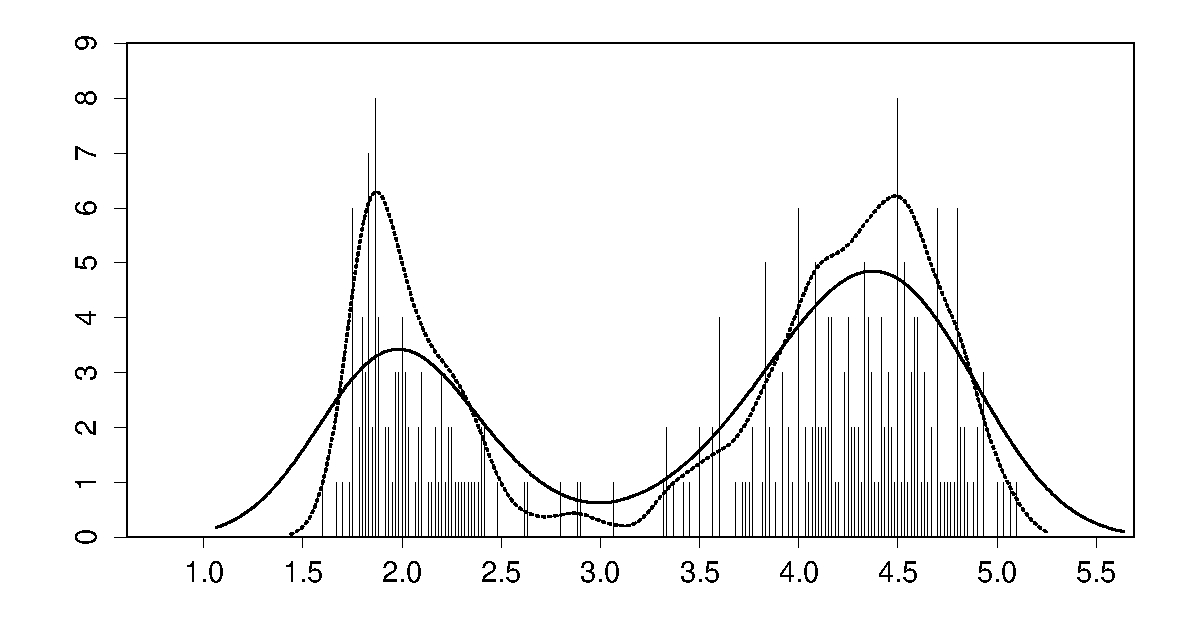
\includegraphics[width=.5\textwidth]{template-files/geys-2kern} %<< no file extension
  %%         --- .5\textwidth stands for 50% of text width
  \caption[Geyser data: binned histogram, Silverman's and another
    kernel]%<<-- Legend for the list of figures at the beginning of you thesis
  {Old Faithful Geyser eruption lengths, $n=272$; binned data and two
    (Gaussian) kernel density estimates ($\times 10$) with $h=h^*= .3348$
    and $h= .1$ (dotted).}% legend displayed below the graph.
  \label{fig:geys2}
\end{figure}

\section{To make a proof}
\begin{proof}
  $1 + 1 = 2$
\end{proof}

\section{To include \Rp code}
See information in Appendix~\ref{app:complement}.


\section{Other information}
Put a text between quotes: make sure to use nice quotes, such as `quote'.

Cite an article or book you refer shortly here, and then listed in the bibliography: \cite{ReferenceKey}.
%%--> in file   myReferences.bib  (same directory)
Or mention that \citeauthor{HamF85} (a person) or \citeauthor{StaWW91} (two
persons) have already done quite a bit work.

Referencing a different part of your work: please refer to Appendix~\ref{app:complement}.


%%% Local Variables: 
%%% mode: latex
%%% TeX-master: "MasterThesisSfS"
%%% End: 

%%\include{tex/Chapter...}
\chapter{Summary}
\label{s:Summary}

Summarize the presented work. Why is it useful to the research field or institute?


\section{Future Work}
\label{ss:FutureWork}

Possible ways to extend the work.


%%% Local Variables: 
%%% mode: latex
%%% TeX-master: "MasterThesisSfS"
%%% End: 

%%%%%%%%%%%%%%%%%%%%%%%%%%%%%%%%%%%%%%%%%%%%%%%%%
%%% Bibliography                              %%%
%%%%%%%%%%%%%%%%%%%%%%%%%%%%%%%%%%%%%%%%%%%%%%%%%
\addtocontents{toc}{\vspace{.5\baselineskip}}
\cleardoublepage
\phantomsection
\addcontentsline{toc}{chapter}{\protect\numberline{}{Bibliography}}
\bibliography{myReferences}
%% All books from our library (SfS) are already in a BiBTeX file
%% 'Assbib.bib' (included here as well), using
% \bibliography{myReferences,Assbib}
% ---------------------------------- instead of the above



%%%%%%%%%%%%%%%%%%%%%%%%%%%%%%%%%%%%%%%%%%%%%%%%% 
%%% Appendices (if needed, e.g. for R code)   %%%
%%%%%%%%%%%%%%%%%%%%%%%%%%%%%%%%%%%%%%%%%%%%%%%%%
\addtocontents{toc}{\vspace{.5\baselineskip}}
\appendix
\chapter{Reproducibility}\label{app:reproducibility}

\section{Reproduce Results}
For reproducibility of the whole computations, we refer to our codebase at:\\ \url{https://github.com/LGraz/MasterThesis-Code}\\ In order to reproduce our computations and results, set up the directory as described in the README. The the `YieldMapping' Data used, is published alongside \cite{perichPixelbasedCropYield2022}. Execute the computations via the script \texttt{./shell\_scripts/reproduce.sh} and do not execute the python and R files by hand (unless you follow the order in \texttt{./shell\_scripts/reproduce.sh}). 

\section{R--Package}
We also provide an \texttt{R} package for a general time series correction and interpolation if additional data is available at: \\
\url{https://github.com/LGraz/CorrectTimeSeries} \\
In our case we consider the NDVI time series and the additional data consists of the unused spectral bands.

We recommend installing it via the \texttt{devtools} package by:\\
\texttt{devtools::install\_github("LGraz/CorrectTimeSeries")}

In the following, we shall give a stand-alone example of how the \texttt{R} package can be used:

\lstinputlisting[title= Example of how to use the \texttt{CorrectTimeSeries} package]{tex/misc/CorrectTimeSeries.R}


\chapter{Further Material}

\section{Data and Methods}{
	\subsection{GDD}\label{app:gdd_examples}
		\cite{baileyUsingGrowingDegree2018} tabulates the corresponding GDD for each stage of wheat.
		\begin{table}[H]
			\centering
			\small
			\begin{tabular}{p{0.2\linewidth} p{0.57\linewidth}  p{0.13\linewidth}} 
				\toprule
				Stage  & Description    & GDD \\
				\hline Emergence & Leaf tip just emerging from above-ground coleoptyle. & $125-160$ \\
				\hline Leaf development & Two leaves unfolded. & $169-208$ \\
				\hline Tillering & First tiller visible  & $369-421$ \\
				\hline Stem elongation & First node detectable. & $592-659$ \\
				\hline Anthesis & Flowering commences; first anthers of cereals are visible. & $807-901$ \\
				\hline Seed fill & Seed fill begins. Caryopsis of cereals watery ripe (first grains have reached half of their final size). & $1068-1174$ \\
				\hline Dough stage & Soft dough stage, grain contents soft but dry, fingernail impression does not hold. & $1434-1556$ \\
				\hline Maturity complete & Grain is fully mature and drydown begins. Ready for harvest when dry. & $1538-1665$ \\
				\bottomrule
			\end{tabular}
		\end{table}
}


\section{Interpolation}
\begin{my_figure}[H]{width=1\textwidth}{interpol/2x3_loess_robust}
	\caption{The LOESS smoother \RobItPlot}
	\label{fig:interpol/2x3_loess_robust}
\end{my_figure}

\begin{my_figure}[H]{width=1\textwidth}{interpol/2x3_B-Splines_robust}
	\caption{B-splines \RobItPlot}
	\label{fig:interpol/2x3_B-Splines_robust}
\end{my_figure}

\begin{my_figure}[H]{width=1\textwidth}{interpol/2x3_DL_robust}
	\caption{A Double Logistic curve \RobItPlot}
	\label{fig:interpol/2x3_DL_robust}
\end{my_figure}

% \subsection{Skewness of LOOCV residuals}
% \begin{my_figure}[h]{width=0.6\textwidth}{interpol/res_cv}
% 	\caption{XXX caption XXX}
% 	\label{fig:interpol/res_cv}
% \end{my_figure}


\section{NDVI correction}
\todo[inline]{page breaks}

% step_plot/2017-201_ndvi.pdf 
% step_plot/2017-202_itpl.pdf 
% step_plot/2017-203_itpl_rew.pdf 
% step_plot/2017-204_ndvi_scl.pdf 
% step_plot/2017-205_show_res.pdf 
% step_plot/2017-206_corr.pdf 
% step_plot/2017-207_uncert.pdf 
% step_plot/2017-208_corr_itpl_rew.pdf

\begin{figure}[H]
	% \vspace{-15pt}
	% \centering
	% \begin{subfigure}[b]{0.42\textwidth}
	% 	\centering
	% 	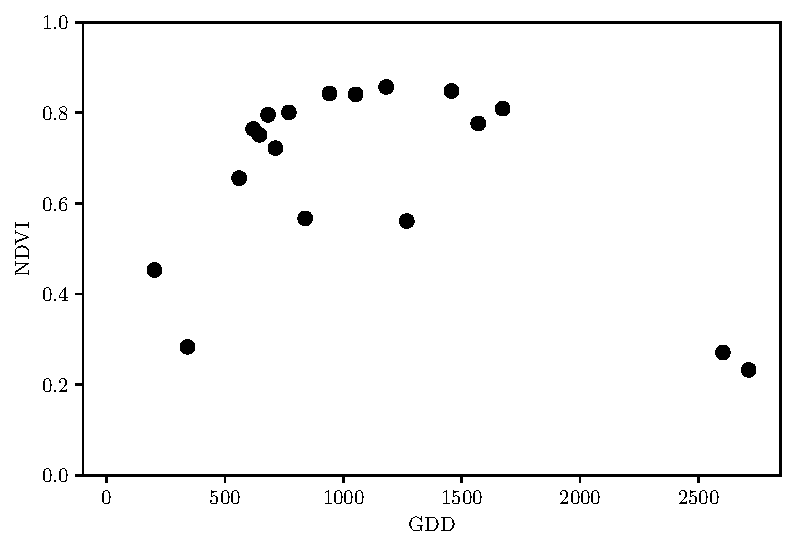
\includegraphics[width=\textwidth]{step_plot/2017-201_ndvi.pdf}
	% 	\vspace{-20pt}
	% 	\caption[NDVI {TS} with SCL45]%
	% 	{{\footnotesize NDVI {TS} with SCL45}}    
	% 	\label{fig:step_plot/2017-201_ndvi.pdf}
	% \end{subfigure}
	% \hfill
	
	\vskip\baselineskip
	\begin{subfigure}[b]{0.42\textwidth}  
		\centering 
		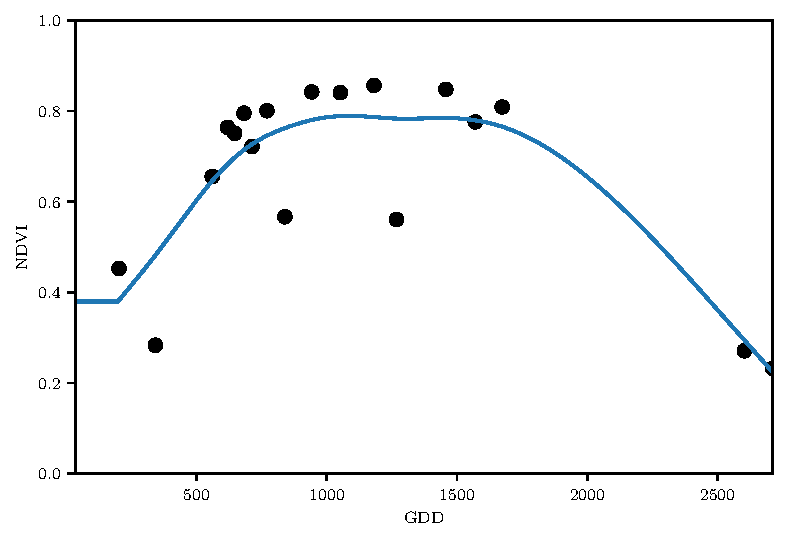
\includegraphics[width=\textwidth]{step_plot/2017-202_itpl.pdf}
		\vspace{-20pt}
		\caption[Interpolation via SS (only SCL45)]%
		{{\footnotesize Interpolation via SS (only SCL45)}}    
		\label{fig:step_plot/2017-202_itpl.pdf}
	\end{subfigure}
	% \begin{subfigure}[b]{0.42\textwidth}   
	% 	\centering 
	% 	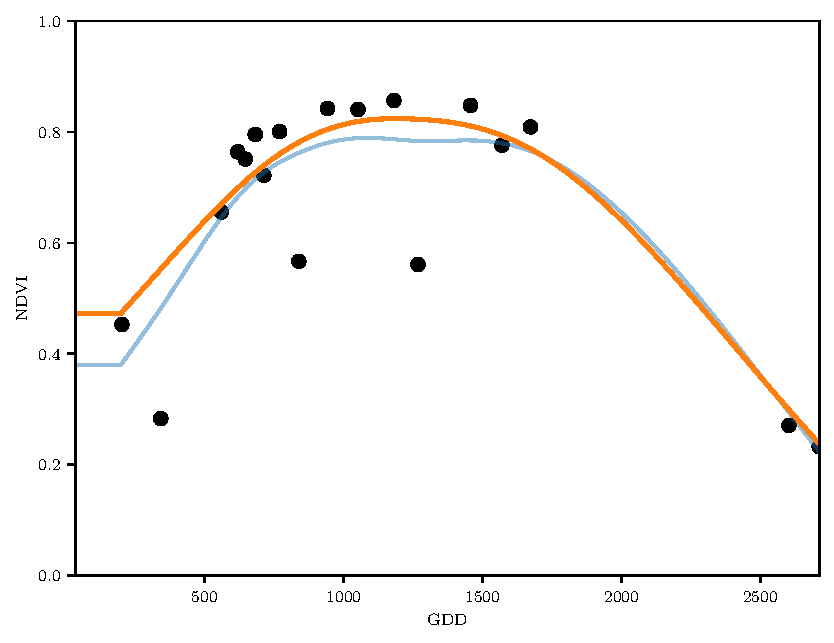
\includegraphics[width=\textwidth]{step_plot/2017-203_itpl_rew.pdf}
	% 	\vspace{-20pt}
	% 	\caption[Robustly reweighted fit]%
	% 	{{\footnotesize Robustly reweighted fit}}    
	% 	\label{fig:step_plot/2017-203_itpl_rew.pdf}
	% \end{subfigure}
	\hfill
	\begin{subfigure}[b]{0.42\textwidth}   
		\centering 
		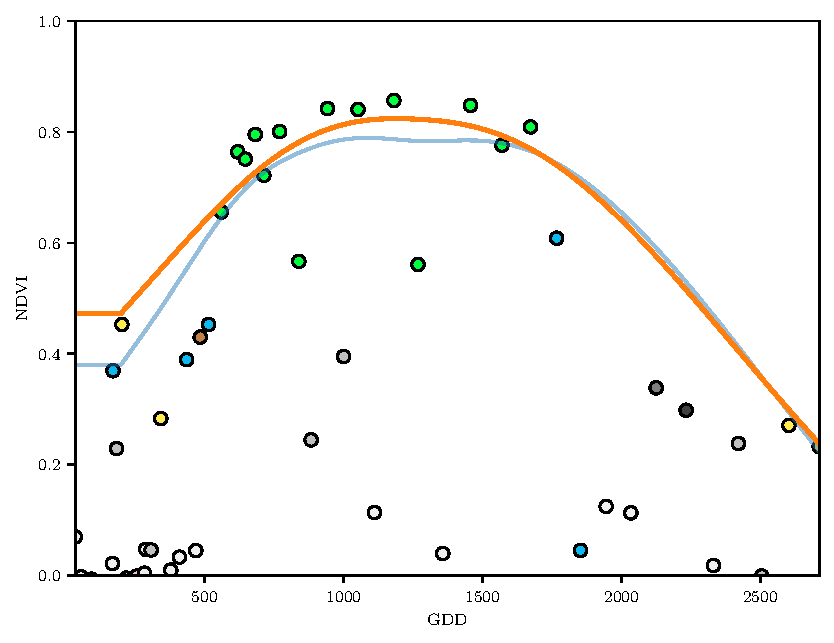
\includegraphics[width=\textwidth]{step_plot/2017-204_ndvi_scl.pdf}
		\vspace{-20pt}
		\caption[Now also consider other SCL-classes]%
		{\footnotesize Now also consider other SCL-classes}    
		\label{fig:step_plot/2017-204_ndvi_scl.pdf}
	\end{subfigure}

	\vskip\baselineskip
	\begin{subfigure}[b]{0.42\textwidth}   
		\centering 
		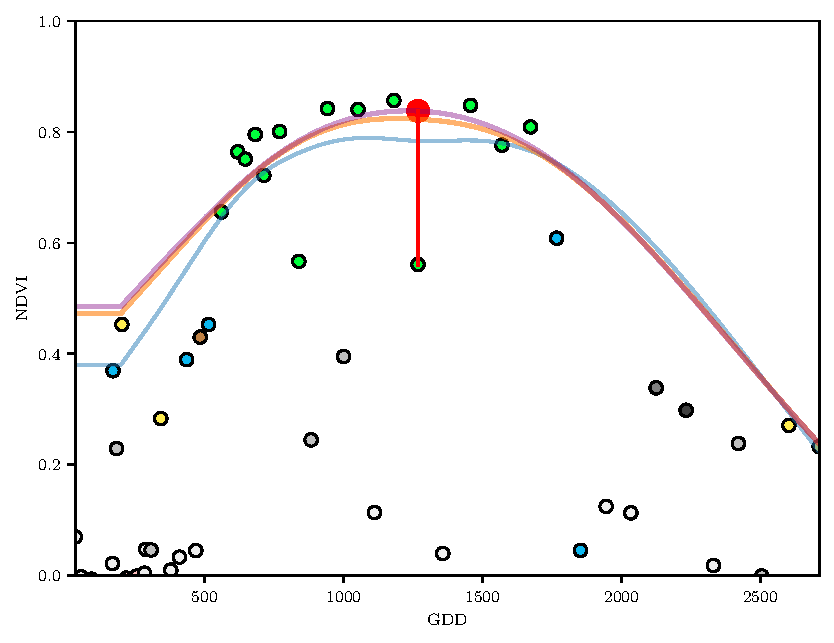
\includegraphics[width=\textwidth]{step_plot/2017-205_show_res.pdf}
		\vspace{-20pt}
		\caption[OOB estim. for each point using SCL45]%
		{{\footnotesize OOB estim. for each point using SCL45}}    
		\label{fig:step_plot/2017-205_show_res.pdf}
	\end{subfigure}
	\hfill
	\begin{subfigure}[b]{0.42\textwidth}   
		\centering 
		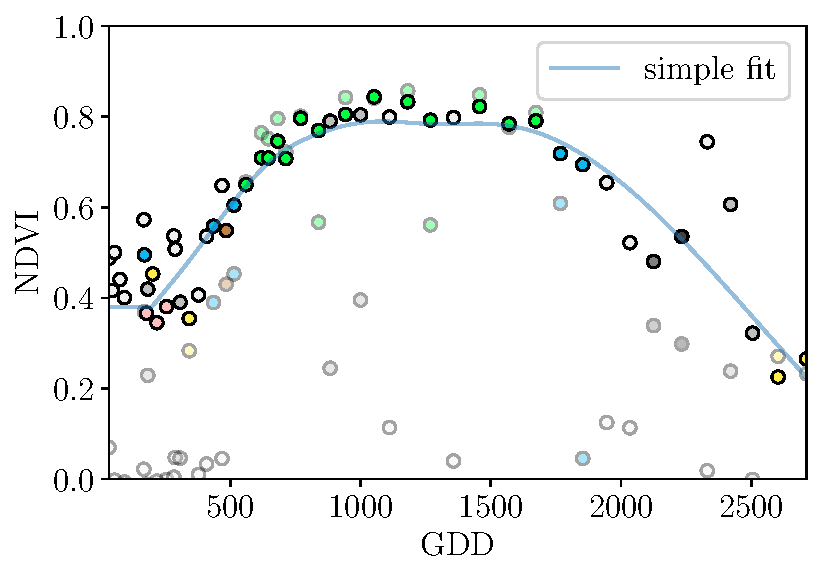
\includegraphics[width=\textwidth]{step_plot/2017-206_corr.pdf}
		\vspace{-20pt}
		\caption[Correct NDVI]%
		{\footnotesize Correct NDVI}    
		\label{fig:step_plot/2017-206_corr.pdf}
	\end{subfigure}

	\vskip\baselineskip
	\begin{subfigure}[b]{0.42\textwidth}   
		\centering 
		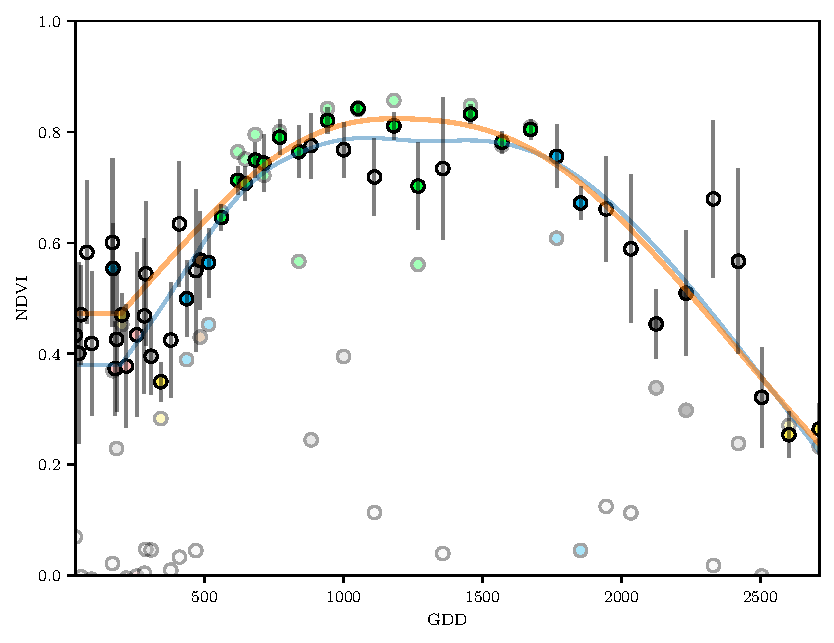
\includegraphics[width=\textwidth]{step_plot/2017-207_uncert.pdf}
		\vspace{-20pt}
		\caption[Estimate absolute errors]%
		{{\footnotesize Estimate absolute errors via statistical model}}    
		\label{fig:step_plot/2017-207_uncert.pdf}
	\end{subfigure}
	\hfill
	\begin{subfigure}[b]{0.42\textwidth}   
		\centering 
		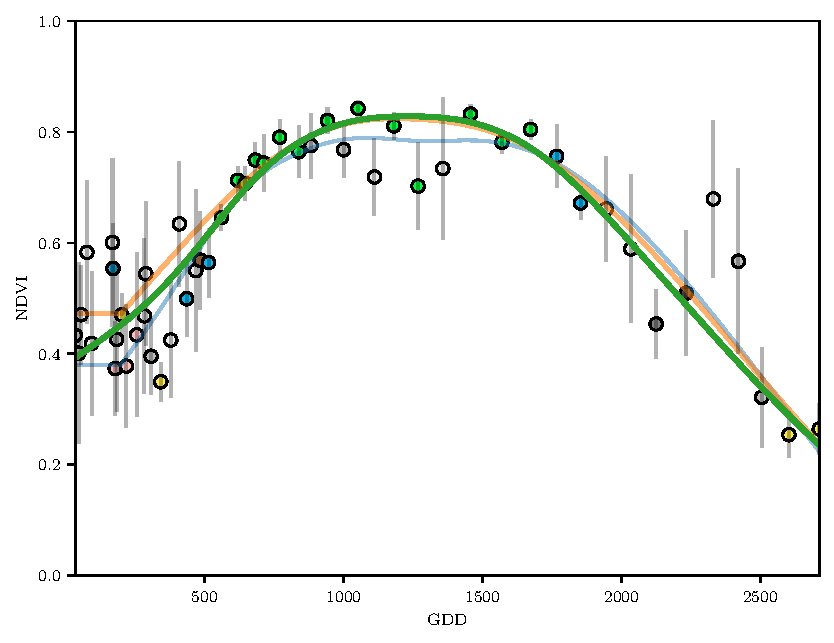
\includegraphics[width=\textwidth]{step_plot/2017-208_corr_itpl_rew.pdf}
		\vspace{-20pt}
		\caption[Interpolation (SS) on weights derived from uncertainties.]%
		{\footnotesize Robust interpolation on weights derived from uncertainties.}    
		\label{fig:step_plot/2017-208_corr_itpl_rew.pdf}
	\end{subfigure}
	\caption[Stepwise illustration of robust NDVI-Correction.]{Stepwise illustration of robust NDVI-Correction. For the color encoding of the SCL classes we refer to table~\ref{tab:satelite/scl_classes}.}
	\label{fig:step_plot_ndvi_corr}
\end{figure}


\begin{table}[H]
	\begin{center}
		\caption{Non-relative RMSE for yield prediction}.
		\small
		\begin{tabular}{lrrrrrrr}
\toprule
 & RF & OLS-SCL & OLS-all & MARS & GAM & LASSO & no-correction \\
\midrule
ss & {\cellcolor[HTML]{000000}} \color[HTML]{F1F1F1} 1.144 & {\cellcolor[HTML]{F1F1F1}} \color[HTML]{000000} 1.033 & {\cellcolor[HTML]{CACACA}} \color[HTML]{000000} 1.051 & {\cellcolor[HTML]{DDDDDD}} \color[HTML]{000000} 1.042 & {\cellcolor[HTML]{D4D4D4}} \color[HTML]{000000} 1.046 & {\cellcolor[HTML]{DDDDDD}} \color[HTML]{000000} 1.042 & {\cellcolor[HTML]{6A6A6A}} \color[HTML]{F1F1F1} 1.095 \\
dl & {\cellcolor[HTML]{222222}} \color[HTML]{F1F1F1} 1.150 & {\cellcolor[HTML]{ADADAD}} \color[HTML]{000000} 1.115 & {\cellcolor[HTML]{A7A7A7}} \color[HTML]{F1F1F1} 1.116 & {\cellcolor[HTML]{A7A7A7}} \color[HTML]{F1F1F1} 1.116 & {\cellcolor[HTML]{F1F1F1}} \color[HTML]{000000} 1.097 & {\cellcolor[HTML]{EDEDED}} \color[HTML]{000000} 1.098 & {\cellcolor[HTML]{000000}} \color[HTML]{F1F1F1} 1.159 \\
ss-rob & {\cellcolor[HTML]{000000}} \color[HTML]{F1F1F1} 1.144 & {\cellcolor[HTML]{F1F1F1}} \color[HTML]{000000} 1.054 & {\cellcolor[HTML]{A2A2A2}} \color[HTML]{F1F1F1} 1.084 & {\cellcolor[HTML]{878787}} \color[HTML]{F1F1F1} 1.094 & {\cellcolor[HTML]{C3C3C3}} \color[HTML]{000000} 1.072 & {\cellcolor[HTML]{C5C5C5}} \color[HTML]{000000} 1.071 & {\cellcolor[HTML]{8F8F8F}} \color[HTML]{F1F1F1} 1.091 \\
dl-rob & {\cellcolor[HTML]{000000}} \color[HTML]{F1F1F1} 1.159 & {\cellcolor[HTML]{4E4E4E}} \color[HTML]{F1F1F1} 1.128 & {\cellcolor[HTML]{696969}} \color[HTML]{F1F1F1} 1.117 & {\cellcolor[HTML]{F1F1F1}} \color[HTML]{000000} 1.064 & {\cellcolor[HTML]{A8A8A8}} \color[HTML]{F1F1F1} 1.093 & {\cellcolor[HTML]{888888}} \color[HTML]{F1F1F1} 1.105 & {\cellcolor[HTML]{060606}} \color[HTML]{F1F1F1} 1.156 \\
\bottomrule
\end{tabular}

		\label{tab:methods_vs_yieldprediction}
		\normalsize
	\end{center}
\end{table}


\begin{table}[H]
	\begin{center}
		\caption{Coefficient of determination (R\textsuperscript{2}) of yield prediction}
		\small
		\begin{tabular}{lrrrrrrr}
\toprule
 & RF & OLS-SCL & OLS-all & MARS & GAM & LASSO & no-correction \\
\midrule
ss & {\cellcolor[HTML]{F1F1F1}} \color[HTML]{000000} 0.431 & {\cellcolor[HTML]{000000}} \color[HTML]{F1F1F1} 0.486 & {\cellcolor[HTML]{272727}} \color[HTML]{F1F1F1} 0.477 & {\cellcolor[HTML]{141414}} \color[HTML]{F1F1F1} 0.481 & {\cellcolor[HTML]{1C1C1C}} \color[HTML]{F1F1F1} 0.479 & {\cellcolor[HTML]{141414}} \color[HTML]{F1F1F1} 0.481 & {\cellcolor[HTML]{878787}} \color[HTML]{F1F1F1} 0.455 \\
dl & {\cellcolor[HTML]{CFCFCF}} \color[HTML]{000000} 0.427 & {\cellcolor[HTML]{444444}} \color[HTML]{F1F1F1} 0.445 & {\cellcolor[HTML]{4A4A4A}} \color[HTML]{F1F1F1} 0.444 & {\cellcolor[HTML]{4A4A4A}} \color[HTML]{F1F1F1} 0.444 & {\cellcolor[HTML]{000000}} \color[HTML]{F1F1F1} 0.454 & {\cellcolor[HTML]{040404}} \color[HTML]{F1F1F1} 0.453 & {\cellcolor[HTML]{F1F1F1}} \color[HTML]{000000} 0.423 \\
ss-rob & {\cellcolor[HTML]{F1F1F1}} \color[HTML]{000000} 0.431 & {\cellcolor[HTML]{000000}} \color[HTML]{F1F1F1} 0.475 & {\cellcolor[HTML]{4E4E4E}} \color[HTML]{F1F1F1} 0.461 & {\cellcolor[HTML]{6A6A6A}} \color[HTML]{F1F1F1} 0.456 & {\cellcolor[HTML]{2D2D2D}} \color[HTML]{F1F1F1} 0.467 & {\cellcolor[HTML]{2B2B2B}} \color[HTML]{F1F1F1} 0.467 & {\cellcolor[HTML]{616161}} \color[HTML]{F1F1F1} 0.457 \\
dl-rob & {\cellcolor[HTML]{F1F1F1}} \color[HTML]{000000} 0.423 & {\cellcolor[HTML]{A2A2A2}} \color[HTML]{F1F1F1} 0.439 & {\cellcolor[HTML]{888888}} \color[HTML]{F1F1F1} 0.444 & {\cellcolor[HTML]{000000}} \color[HTML]{F1F1F1} 0.470 & {\cellcolor[HTML]{494949}} \color[HTML]{F1F1F1} 0.456 & {\cellcolor[HTML]{696969}} \color[HTML]{F1F1F1} 0.450 & {\cellcolor[HTML]{EBEBEB}} \color[HTML]{000000} 0.424 \\
\bottomrule
\end{tabular}

		\label{tab:methods_vs_yieldprediction_r2}
		\normalsize
	\end{center}
\end{table}

\subsection{OLS-SCL Model Outputs}\label{app:ols-scl-summary}
\lstinputlisting[title= R Summary of the NDVI correction model (cf. equation \refeq{eq:corr_lm})]{tex/chapters/misc/lm_scl.txt}
\lstinputlisting[title= R Summary of the NDVI correction model (cf. equation \refeq{eq:corr_lm_res})]{tex/chapters/misc/lm_scl_res.txt}


\todo[inline]{replace space before ref by tilda}
\todo[inline]{check quantile definitions}
\todo[inline]{schwarz weiss färbung der IS tabelle korrigieren}
\todo[inline]{so wenig wie möglich abkürzungen in den fig und table captions}
\todo[inline]{refer to data aviability}
\todo[inline]{abkürzungen Fourier und in tabellen}
\todo[inline]{figure spacing (caption zu nah dran --- manuell vspace einfügen wo nötig)}
\todo[inline]{italics für definitionen wie `variogramm' ja/nein --- einheitlich}
\todo[inline]{Gross schreiben von Fussnoten \& tabelleneinträgen + Satzzeichen}

% \chapter{Complementary information}
\label{app:complement}

Additional material. For example long mathematical derivations could be
given in the appendix. Or you could include part of your code that is
needed in printed form. You can add several Appendices to your thesis (as
you can include several chapters in the main part of your work).

\section{Including \Rp code with verbatim}
A simple (rather too simple, see~\ref{App:listings}) way to include code or
  {\it R} output is to use
\texttt{verbatim}. It just prints the text however it is (including all
spaces, ``strange'' symbols,...) in a slightly different font.
\begin{verbatim}
## loading packages
library(RBGL)
library(Rgraphviz)
library(boot)

## global variables
X_MAX <- 150

   This allows me to put as many s  p a   c es   as I want.
I can also use \ and ` and & and all the rest that is usually only 
accepted in the math mode.

I can also make as 
                  many 
             line 
    breaks as 
I want... and
             where I want. 
\end{verbatim}

But really recommended,  much better is the following:

\section{Including \Rp code with the \emph{listings} package}\label{App:listings}
However, it is much nicer to use the \emph{listings} package to include \Rp
code in your report. It allows you to number the lines, color the comments
differently than the code, and so on.
All the following is produced by simply writing
\verb! \lstinputlisting{figures/template-files/picture.R} !  in your \LaTeX\ ``code'':

\lstinputlisting{figures/template-files/picture.R}

or \verb!\lstinputlisting{/u/maechler/R/Pkgs/sfsmisc/R/misc/ellipse.R}! :

\lstinputlisting{misc/ellipse.R}% was /u/maechler/R/Pkgs/sfsmisc/R/misc/ellipse.R

\section{Using \texttt{Sweave} (or \texttt{knitr}) to include \Rp code (and more) in your report}
The easiest (and most elegant) way to include \Rp code and its output (and
have all your figures up to date with your report) is to use Sweave---or the
\href{https://cran.R-project.org/package=knitr}{\texttt{knitr}} R package with even more possibilities.
% You can find an introduction Sweave in \texttt{/u/sfs/StatSoftDoc/Sweave/Sweave-tutorial.pdf}.

Search the web to find lots of intro material on how to use Sweave or
\href{https://en.wikipedia.org/wiki/Knitr}{knitr (on Wikipedia)}.

%%% Local Variables: 
%%% mode: latex
%%% TeX-master: "MasterThesisSfS"
%%% End: 

% \chapter{Yet another appendix....}

\section{Description}
\begin{description}
\item[Something] details.
\item[Something else] other definition.
\end{description}

\section{Tables}
Refer to Table~\ref{tab:example} to see a left justified table with caption
on top.

\begin{table}[ht]
\centering
\caption[Test results]{\label{tab:example}Results.}
\begin{tabular}{ll}
\hline
\textbf{Student} & \textbf{Grade}\\
\hline
Marie  & $6$\\
Alain  & $5.5$\\
Josette  & $4.5$\\
Pierre  & $5$\\
\hline
\end{tabular}
\end{table}

%%% Local Variables: 
%%% mode: latex
%%% TeX-master: "MasterThesisSfS"
%%% End: 

% \chapter{2nd Appendix: More sophisticated R code listing} \label{appendix-more-R}

Chapter-wise listing of parts of R code, using
\begin{itemize}
\item \texttt{firstline=n1}
\item \texttt{lastline=n2}
\item \texttt{title=<text>}
\end{itemize}
e.g., for the first example below
\begin{verbatim}
\lstinputlisting[firstline=1,lastline=32,
                 title= \texttt{read\_irwls\_fn.R}]{../RCode/read_irwls_fn.R}
\end{verbatim}

% \section{Chapter 2} \label{app 2}

% \lstinputlisting[firstline=1,lastline=77,
% title=\texttt{analytic\_efficiency.R}]{../RCode/analytic_efficiency.R}
% %\lstinputlisting[firstline=,lastline=]{../RCode/???.R}

\bigskip% or even  \clearpage

%-----------------------------------------------------------------------------------------
\section{Chapter 5} \label{app 5}

% \lstinputlisting[firstline=1,lastline=71,
%                  title=\texttt{loss-fn\_rotated.R}]{../RCode/loss-fn_rotated.R}
\lstinputlisting[firstline=1,lastline=32,
                 title= \texttt{read\_irwls\_fn.R}]{misc/ellipse.R}

\medskip
                 
\lstinputlisting[firstline=1,lastline=45,
                 title=\texttt{plot.psi.R}]{misc/ellipse.R}
%\lstinputlisting[firstline=,lastline=]{../RCode/???.R}
%\lstinputlisting[firstline=,lastline=]{../RCode/???.R}

% \clearpage
%-----------------------------------------------------------------------------------------
% \section{Chapter 7} \label{app 7}

% \lstinputlisting[firstline=1,lastline=35,
%                  title= \texttt{stat.test} from \texttt{lmrob2-fn.R}]{../RCode/lmrob2-fn.R}
% \lstinputlisting[firstline=41,lastline=194,
%                  title=\texttt{M.optimal.ms} from \texttt{lmrob2-fn.R}]{../RCode/lmrob2-fn.R}
%\lstinputlisting[firstline=,lastline=]{../RCode/???.R}
%-----------------------------------------------------------------------------------------

%%% Local Variables:
%%% mode: latex
%%% TeX-master: "MasterThesisSfS"
%%% End:


\ifdraft \else %XXX
  % %% Epilogue (optional)
  % \addtocontents{toc}{\vspace{.5\baselineskip}}
  % \cleardoublepage
  % \phantomsection
  % \addcontentsline{toc}{chapter}{\protect\numberline{}{Epilogue}}
  % \markboth{Epilogue}{Epilogue}
  % \chapter*{Epilogue}
\label{s:Epilogue}

A few final words.



%%% Local Variables: 
%%% mode: latex
%%% TeX-master: "MasterThesisSfS"
%%% End: 



  %%%%%%%%%%%%%%%%%%%%%%%%%%%%%%%%%%%%%%%%%%%%%%%%%% 
  %%% Declaration of originality (Do not remove!)%%%
  %%%%%%%%%%%%%%%%%%%%%%%%%%%%%%%%%%%%%%%%%%%%%%%%%%
  %% Instructions:
  %% -------------
  %% fill in the empty document confirmation-originality.pdf electronically
  %% print it out and sign it
  %% scan it in again and save the scan in this directory with name
  %% confirmation-originality-scan.pdf 
  %%
  %% General info on plagiarism:
  %% https://www.ethz.ch/students/en/studies/performance-assessments/plagiarism.html 
  \cleardoublepage
  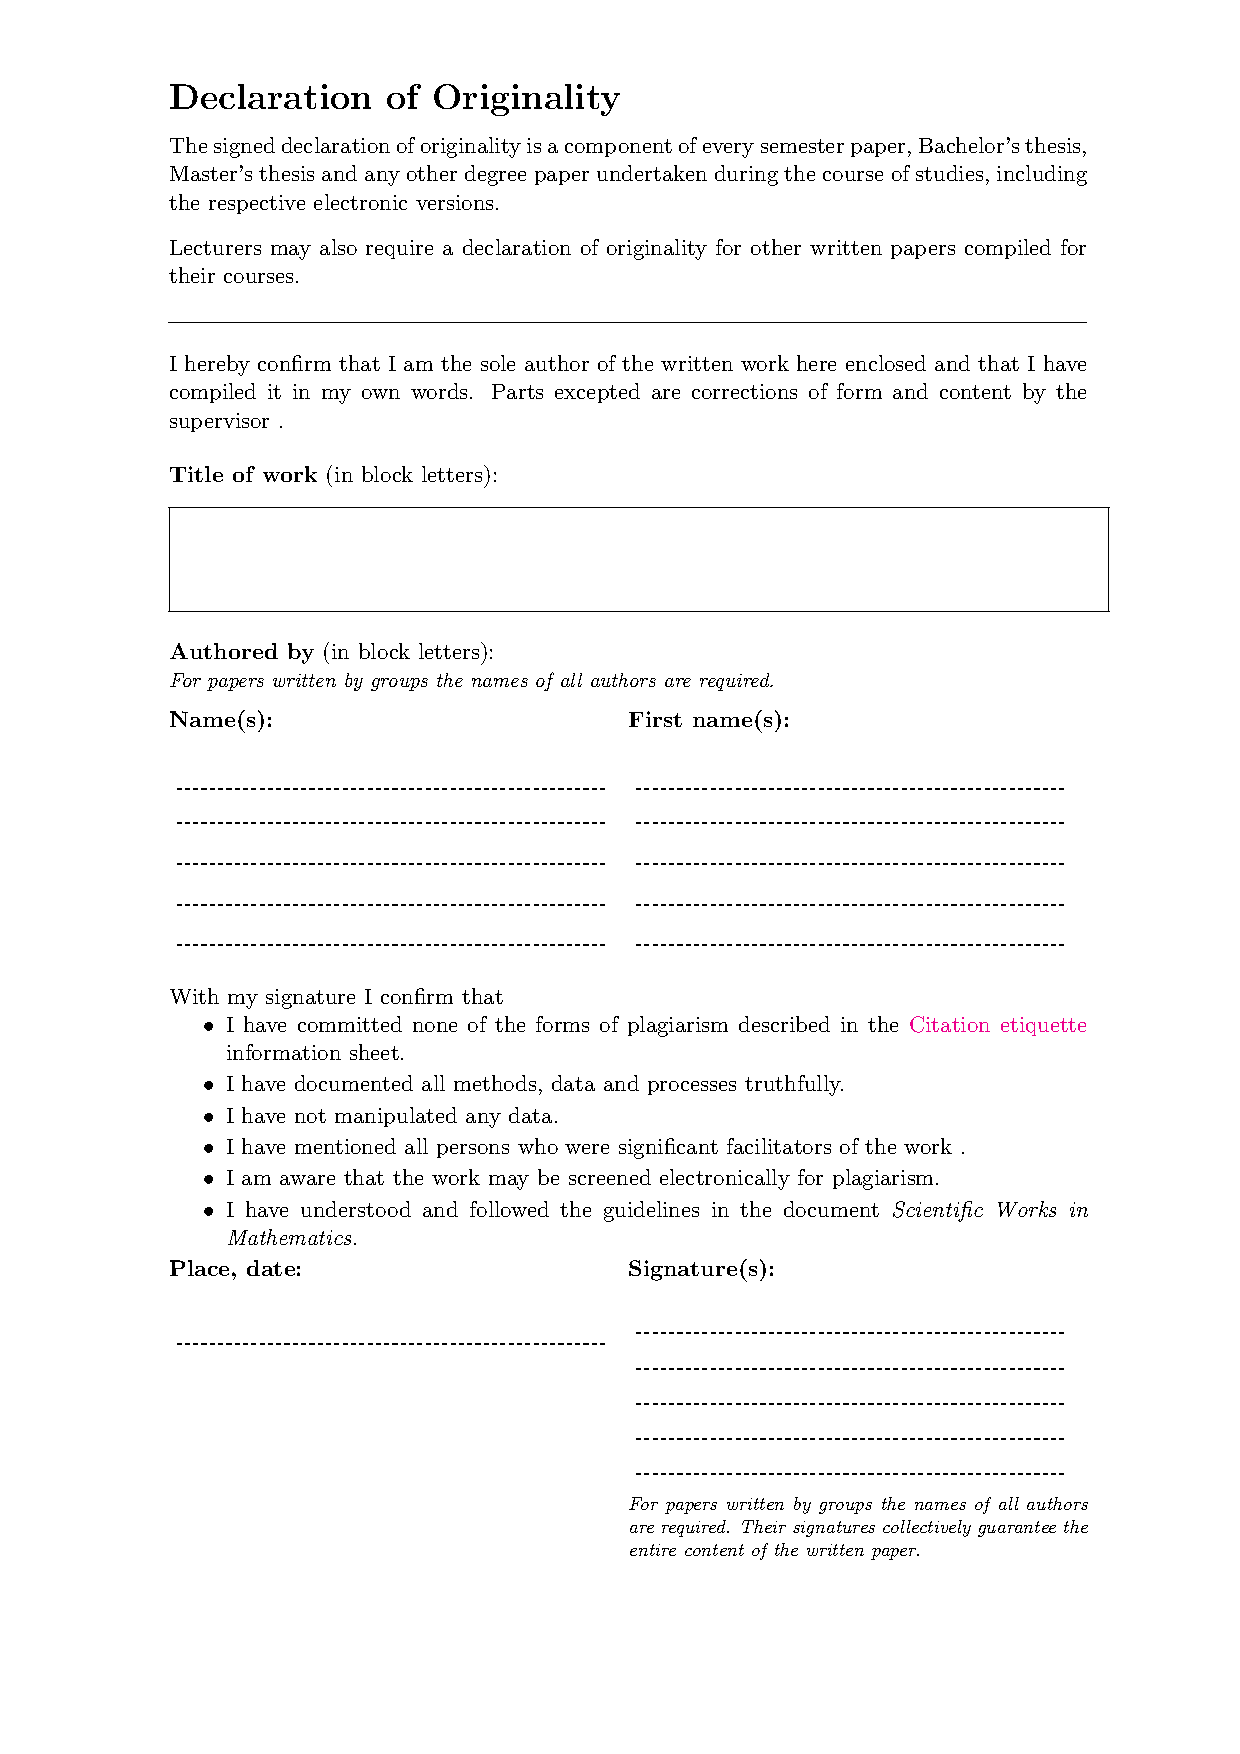
\includepdf[pages={-}, frame=true,scale=1]{misc/confirmation-originality.pdf}
\fi
\end{document}

%%% Local Variables:
%%% mode: latex
%%% TeX-master: "MasterThesisSfS"
%%% End:
